% !TeX root = ../main.tex


\begin{wrapfigure}{r}{0.3\textwidth}
  \centering
  \vspace{-3ex}
  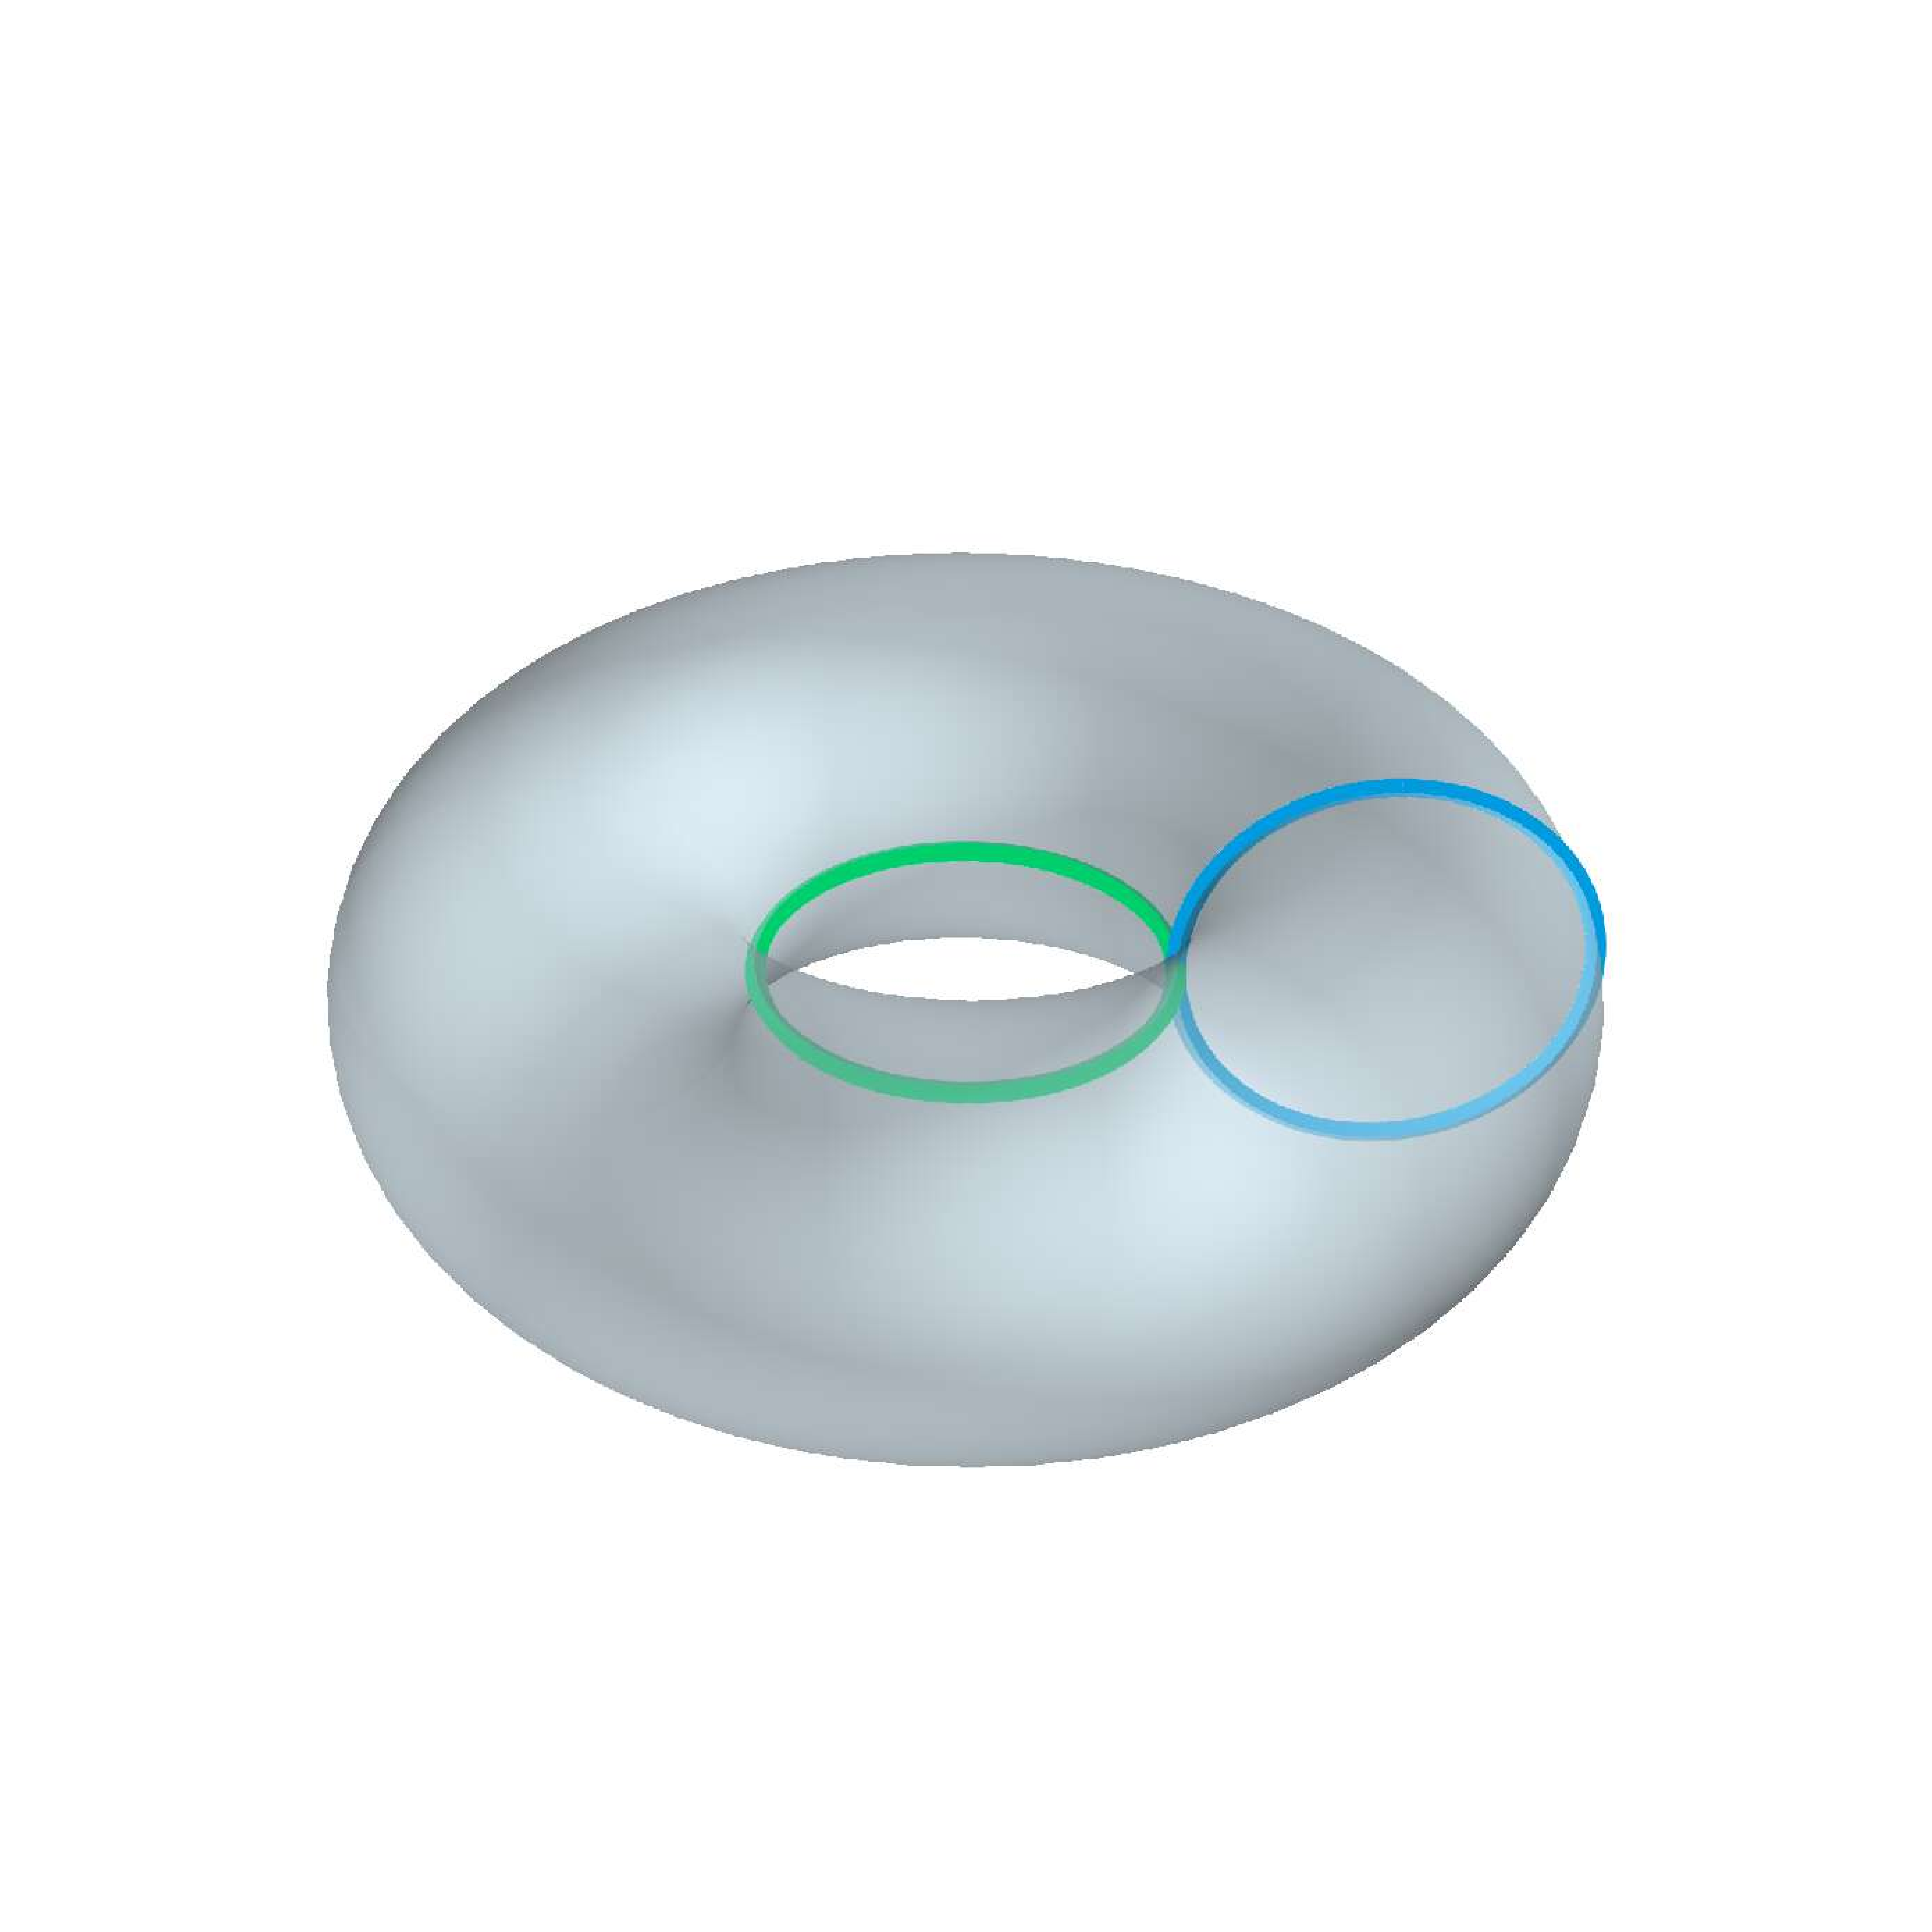
\includegraphics[trim=300 400 300 400, clip, width=\linewidth]{figures/torus1_light-comp.pdf}
    \caption{The 2-Torus has one component, two loops (representative cycles shown), and one void.}
\end{wrapfigure}

Topology is the mathematical study of shape.
Often referred to as ``rubber sheet geometry,'' topology is concerned with the properties of a space that are invariant under continuous transformations.
Connected components, loops, and voids are examples of topological invariants---holes in dimensions 0, 1, and 2---that are captured by the \emph{homology} of a space.
Homology associates an algebraic structure to a space that can be used to quantify these holes in arbitrary dimension.
Persistent homology uses this structure to decompose the homology of a space through a nested sequence of subspaces~\cite{edelsbrunner02simplification}.
Often, this sequence is defined by a scalar-valued function, with subspaces consisting of points that map to scalar values within some range.
The resulting decomposition provides a topological signature that encodes useful geometric and topological information about the function, as well as the space itself.

\begin{figure}[htbp]
  \begin{minipage}{0.35\textwidth}
    \centering
    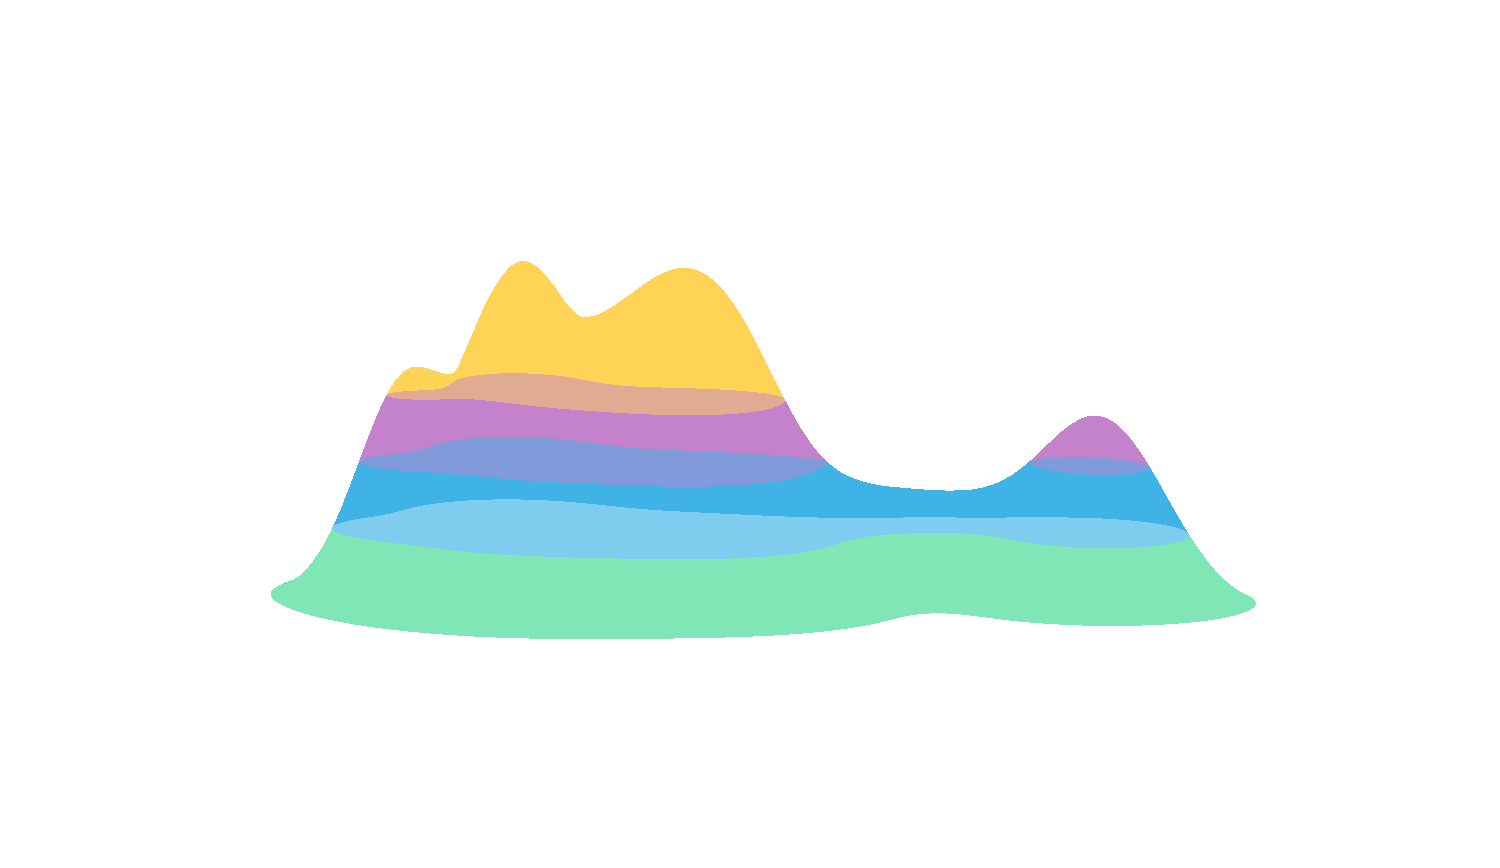
\includegraphics[trim=200 200 200 200, clip, width=0.8\linewidth]{figures/surf-side.png}
    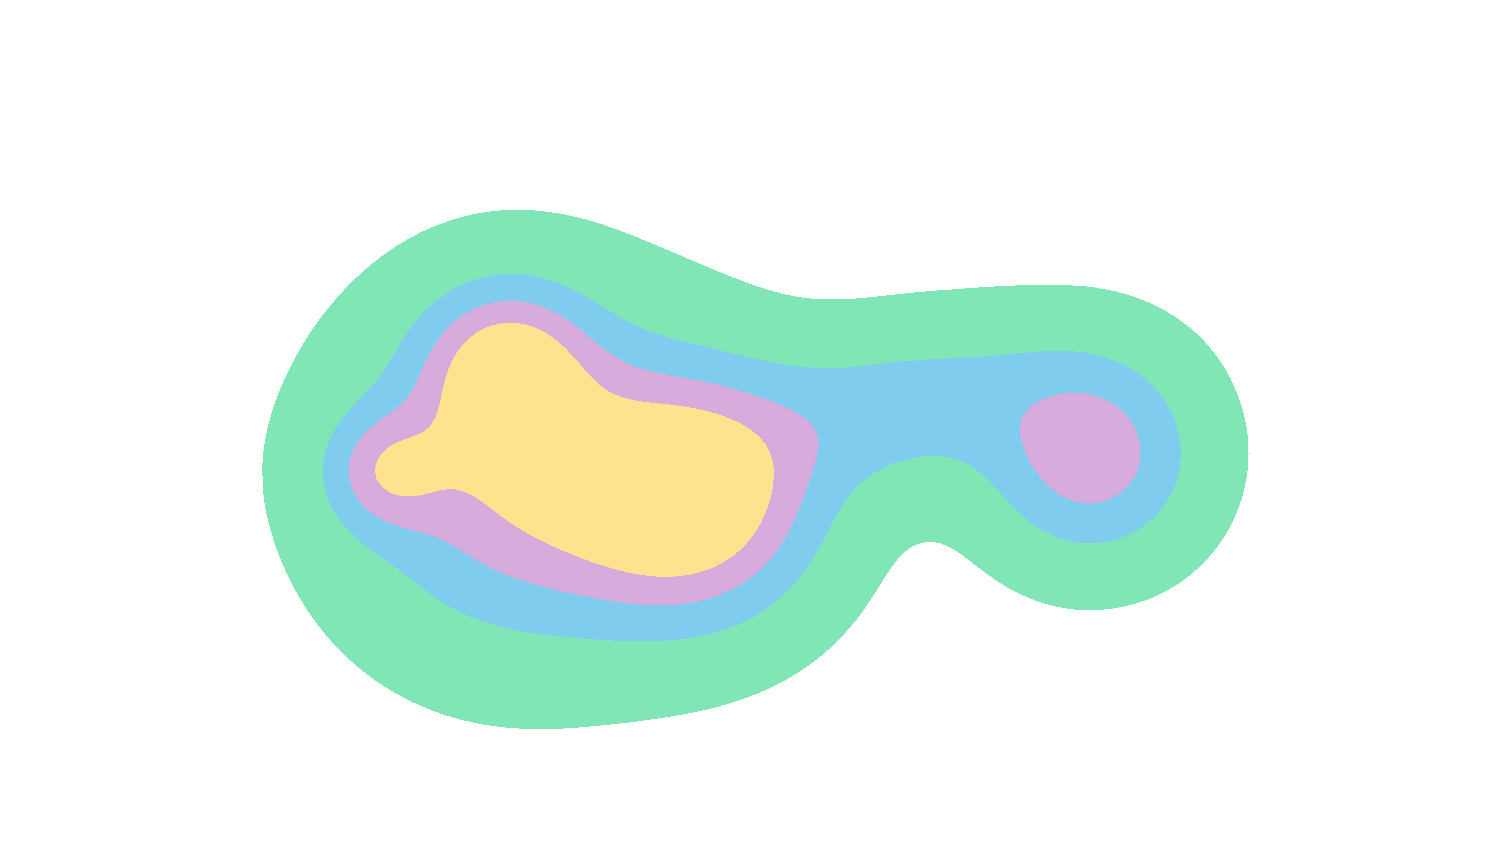
\includegraphics[trim=200 100 200 150, clip, width=0.75\linewidth]{figures/surf-top.png}
  \end{minipage}
  \begin{minipage}{0.5\textwidth}
    \centering
    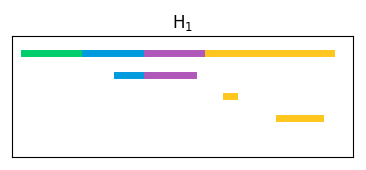
\includegraphics[width=\linewidth]{figures/scalar_barcode_H1.png}
  \end{minipage}
  \caption{A scalar field on a 2D domain and its persistent homology in dimension 1.}
\end{figure}

% \begin{figure}[htbp]
%   \centering
%   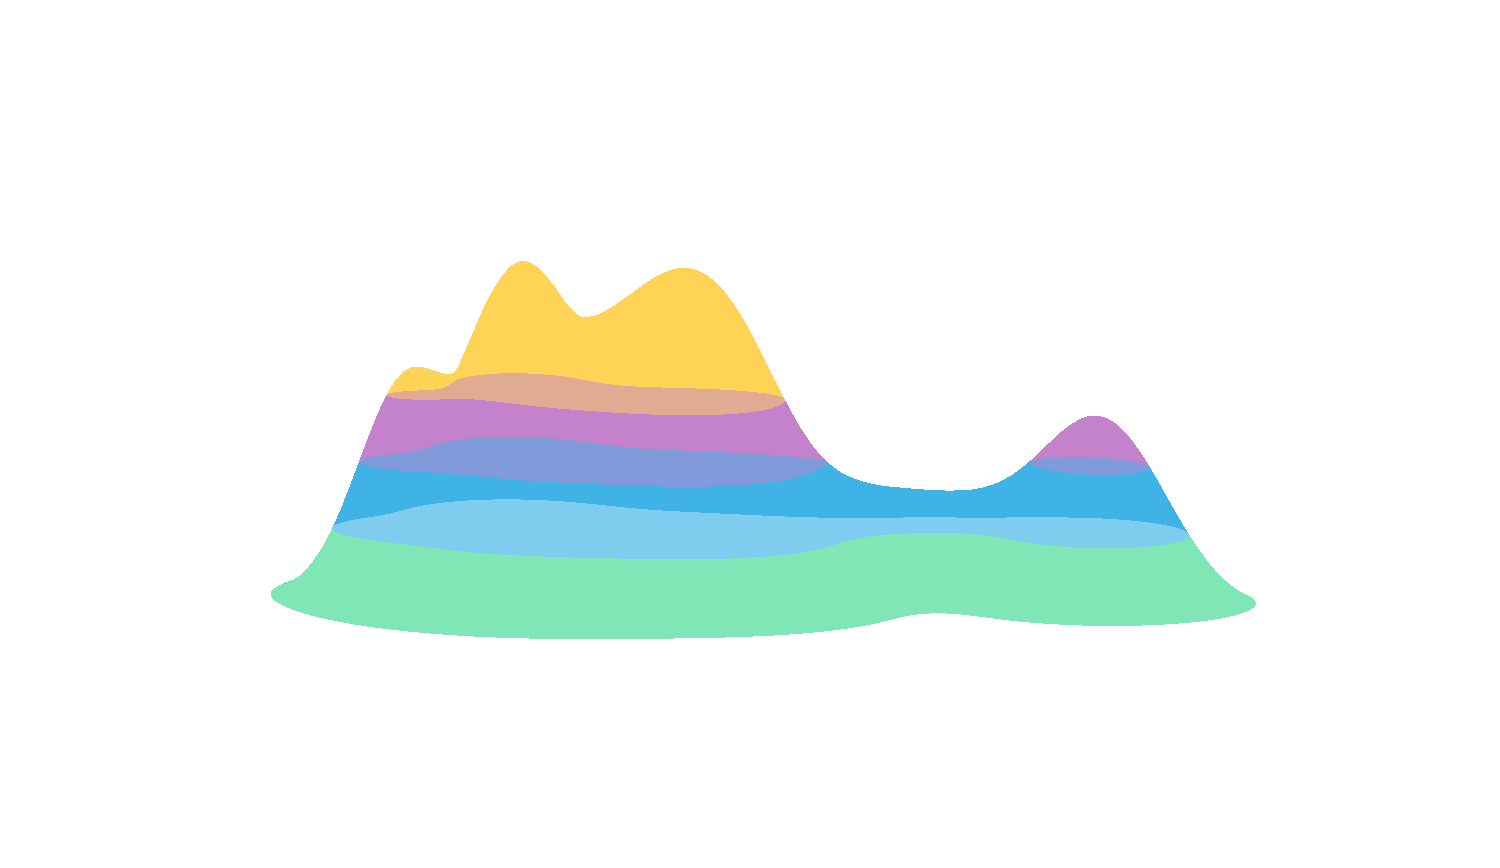
\includegraphics[trim=200 200 200 200, clip, width=0.45\textwidth]{figures/surf-side.png}
%   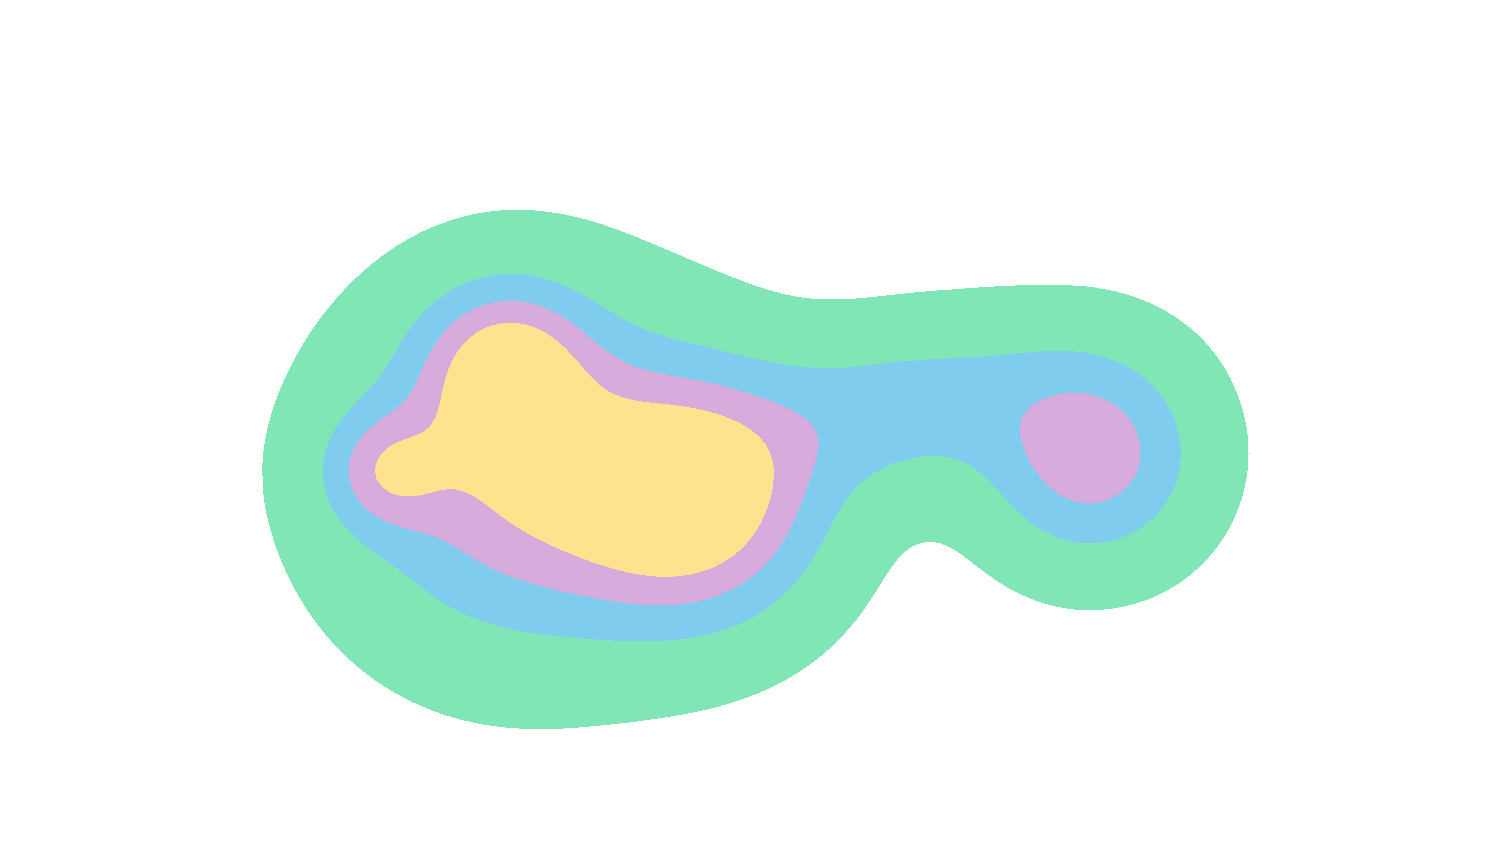
\includegraphics[trim=250 0 50 100, clip, width=0.35\textwidth]{figures/surf-top.png}
%   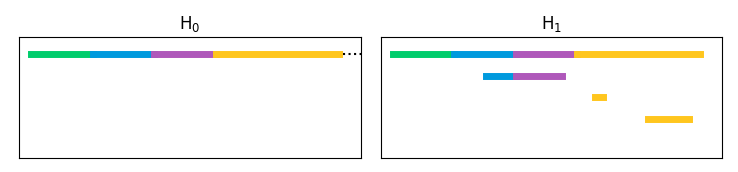
\includegraphics[width=0.75\textwidth]{figures/scalar_barcode_true.png}
%   \caption{A scalar field on a 2D domain and its persistent homology in dimension 0 and 1.}
% \end{figure}

Topological Scalar Field Analysis (SFA) is concerned with approximating the persistent homology of a scalar-valued function, or scalar field, from a finite set of sample points~\cite{chazal09analysis,buchet15topological}.
A fundamental assumption required to have strong guarantees is that the domain of the function is sufficiently well-sampled.
The Topological Coverage Criterion (TCC) is a topological condition for coverage that can be used to confirm that a given sample is sufficient~\cite{desilva06coordinate,desilva07coverage,desilva07homological,cavanna2017when}.
Moreover, the TCC uses much of the same homological and combinatorial tools required for SFA.
In fact, under mild regularity assumptions, coverage can be confirmed directly from the persistent homology a sample approximates.
In this paper, we show how the TCC can be modified so that one can simultaneously approximate the persistent homology of a scalar-valued function while verifying that the domain of the function is sufficiently well-sampled.
Not only does this replace unnatural assumptions made in the TCC, but it also extends SFA to the setting of partial coverage.

% We therefore adapt the TCC to the setting of SFA so that coverage by an arbitrary sample can be confirmed directly from the persistent homology it approximates.
% This is done by considering the persistent homology of the scalar field with respect to a specific subspace.
% Not only does this remove unnatural assumption made in previous work on the TCC, but it also generalizes SFA to the setting of partial coverage.

% \begin{figure}[htbp]
\begin{wrapfigure}{r}{0.4\textwidth}
  \centering
  \vspace{-4ex}
  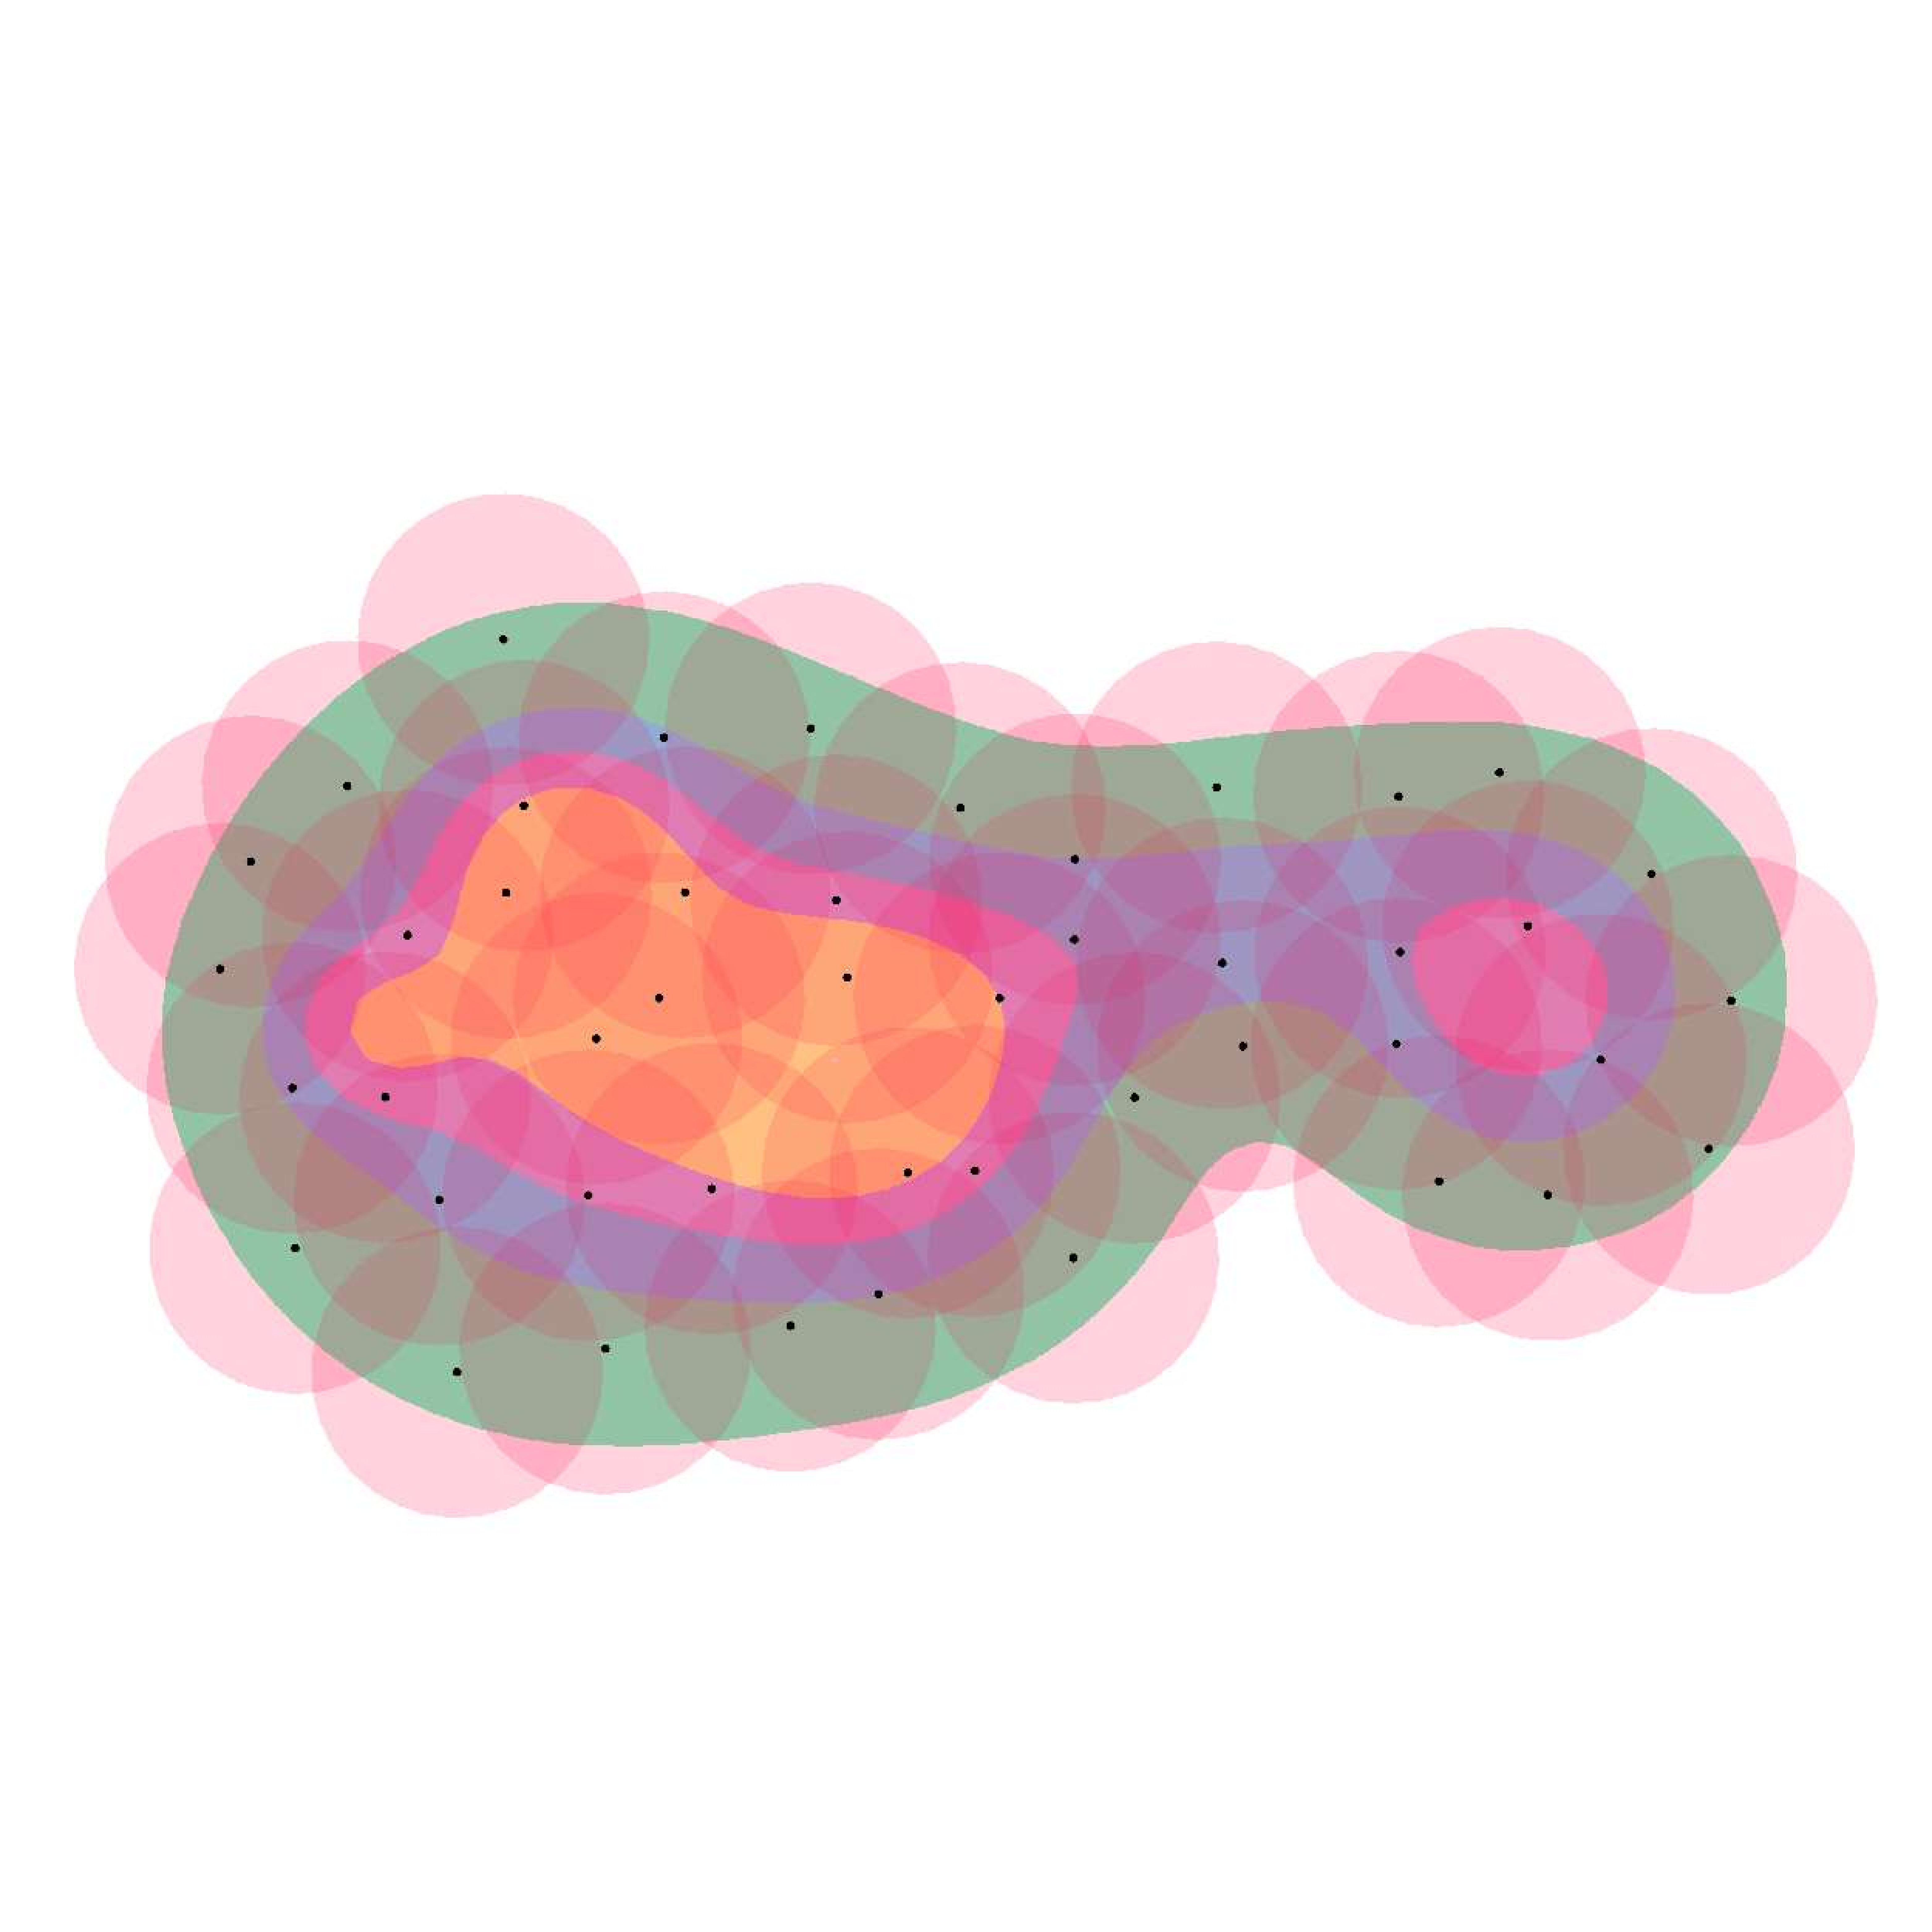
\includegraphics[trim=100 600 100 700, clip, width=\linewidth]{figures/partial4/cover-comp.pdf}
  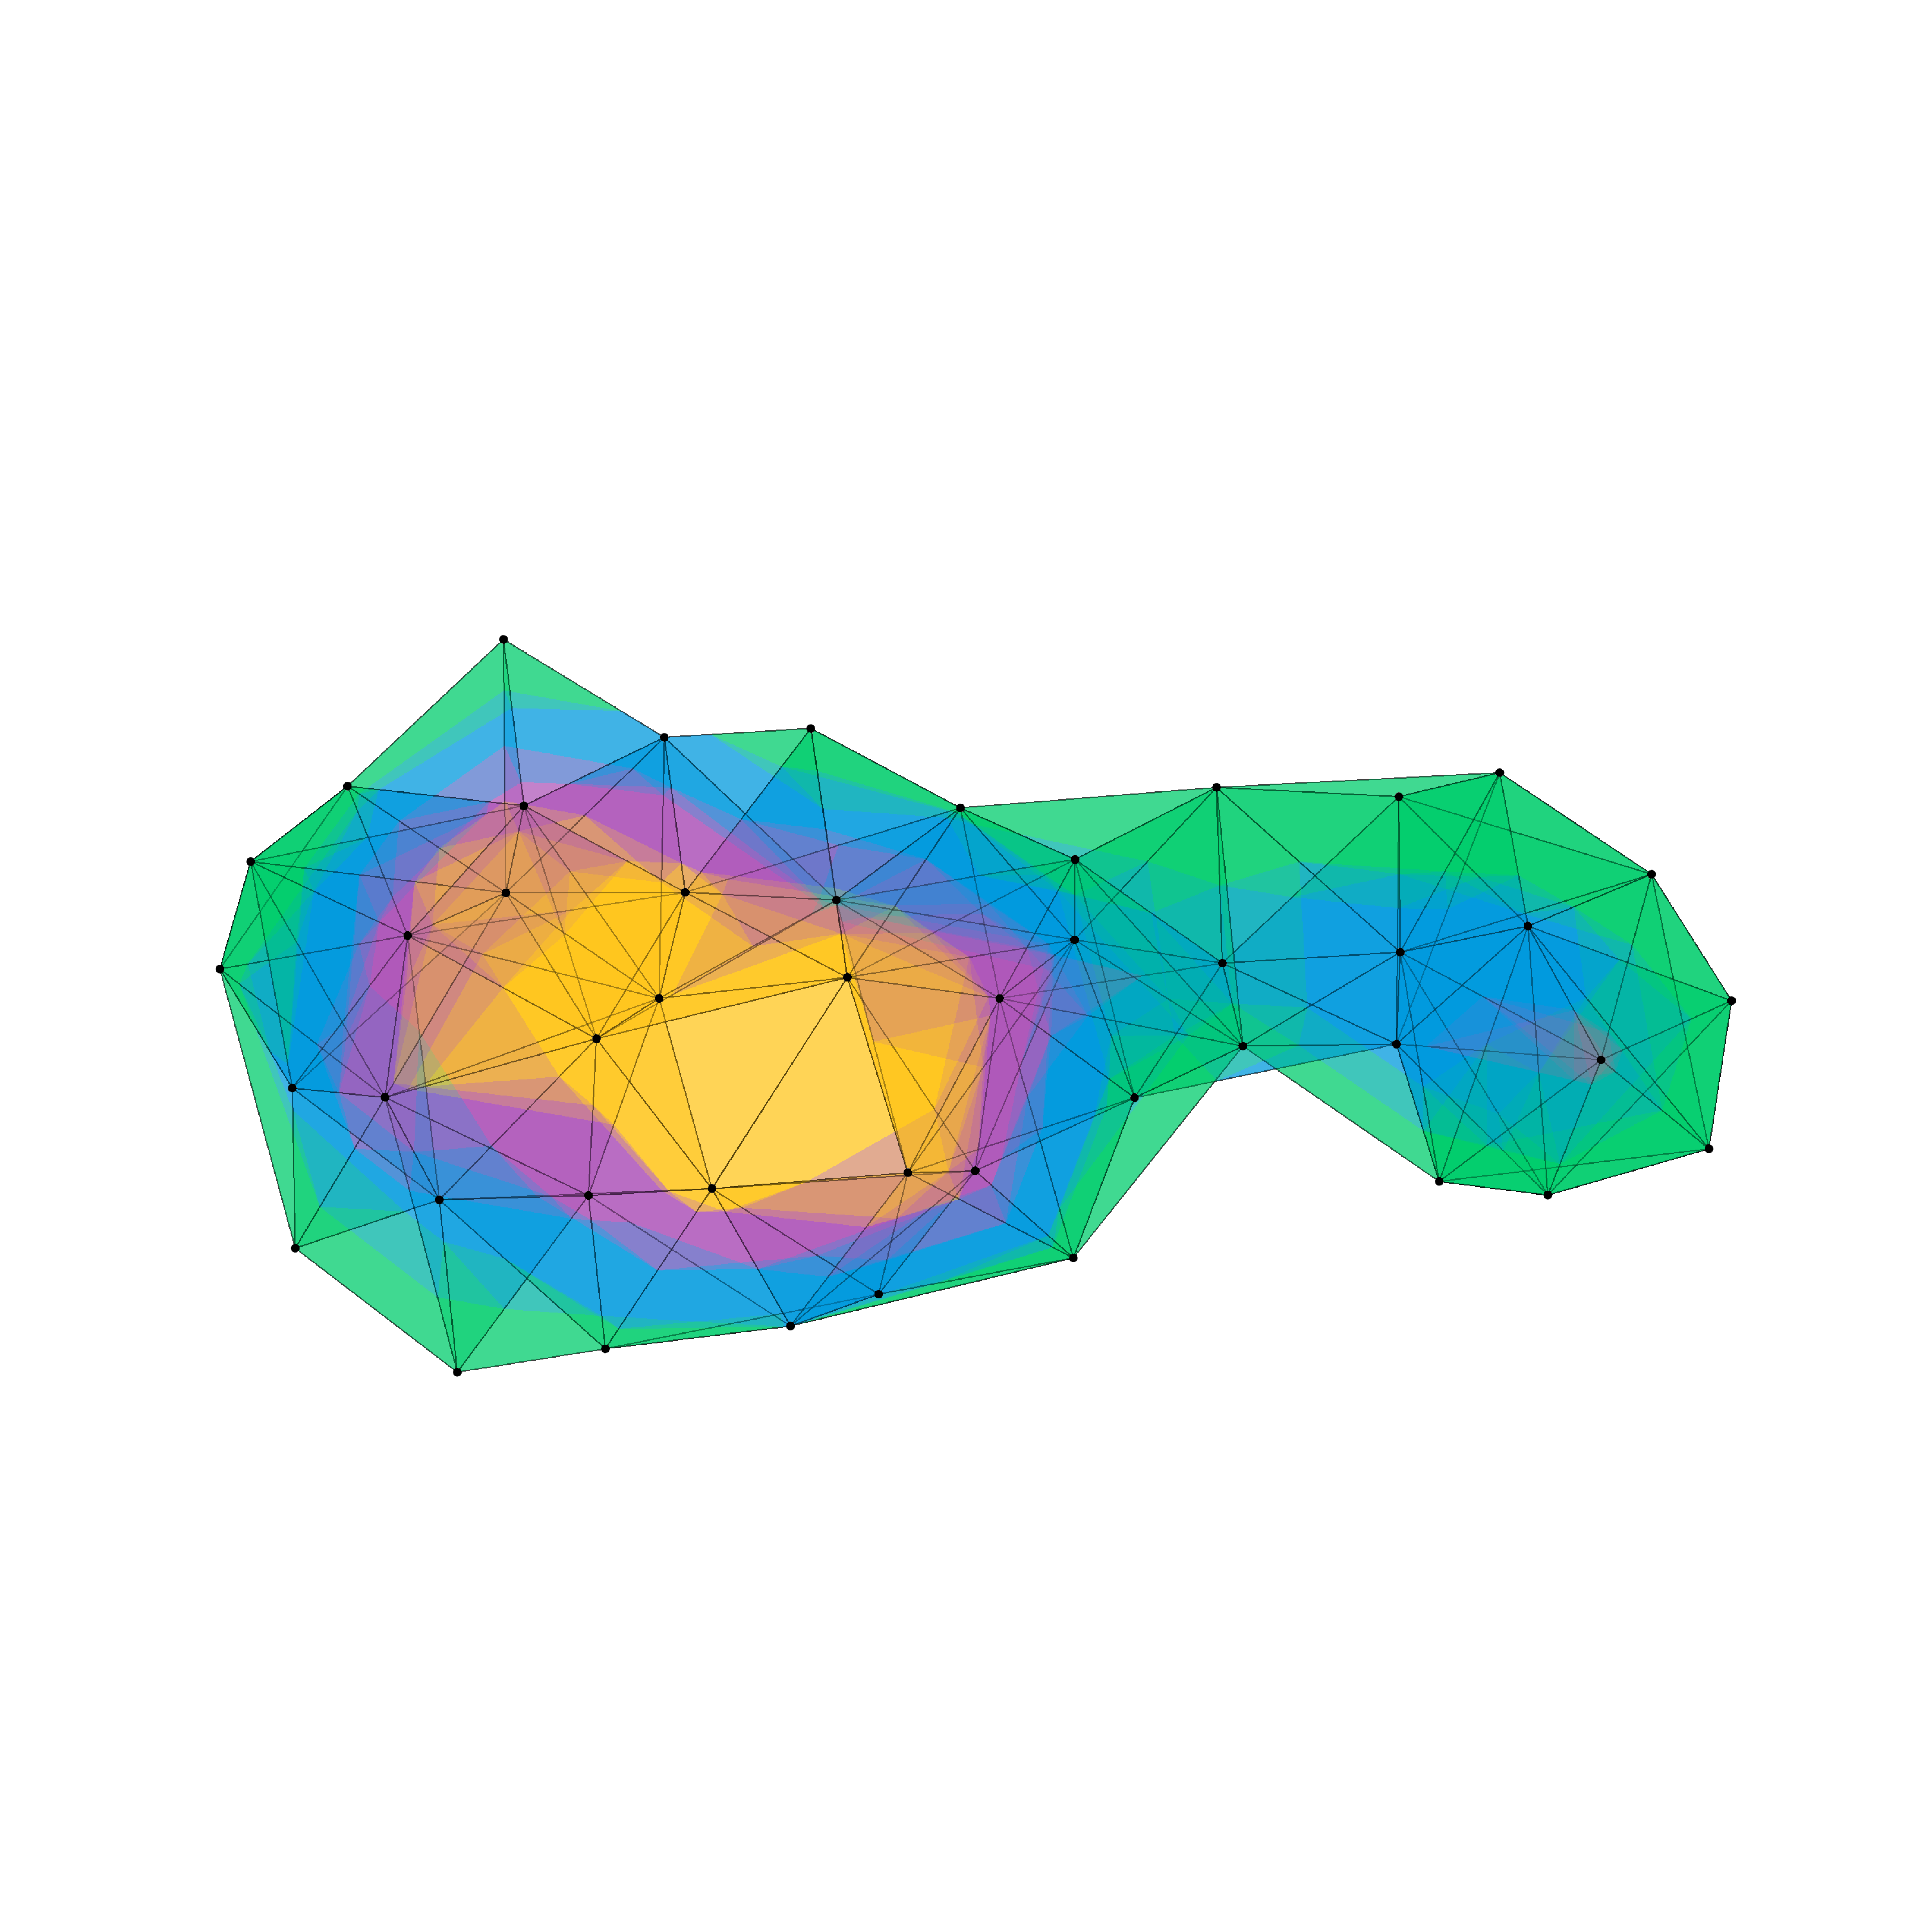
\includegraphics[trim=100 600 100 900, clip, width=\linewidth]{figures/partial4/complex_nosurf.pdf}
  \caption{A cover of a scalar field and a discrete structure used to approximate its persistent homology.}
% \end{figure}
\end{wrapfigure}

\paragraph{Related Work}

% neuroscience~\cite{Giusti_2015,sizemore2016classification,sizemore2018cliques,sizemore2019importance,saggar2018towards},
% structural biology~\cite{xia2014persistent,cang2015topological,dey2018protein,kovacev2016using,gameiro2015topological},
% medical imaging~\cite{adams2009nonlinear,bendich2010computing,carlsson2008local,robins2011theory,bendich2016persistent},
% geometry processing~\cite{carlsson2005persistence,dey2010persistent,poulenard2018topological,skraba2010persistence,bruel2020topology},
% and machine learning~\cite{giansiracusa2017persistent,hofer2017deep,clough2019explicit,chen2019topological,carlsson2020topological,gabrielsson2020topology},

Persistent homology is an important tool in the emerging field of Topological Data Analysis (TDA).
TDA is concerned with the ``shape of data,'' and has found applications in
neuroscience~\cite{saggar2018towards, sizemore2019importance},
structural biology~\cite{gameiro2015topological,kovacev2016using,dey2018protein},
medical imaging~\cite{carlsson2008local,robins2011theory,bendich2016persistent},
geometry processing~\cite{skraba2010persistence,poulenard2018topological,bruel2020topology},
and machine learning~\cite{clough2019explicit,chen2019topological,carlsson2020topological,gabrielsson2020topology}, to name a few.
Topological methods are appealing to data analysis primarily because of their ability to identify meaningful global structure from local, often high dimensional data.
SFA has an important role in TDA as many problems in data analysis require reliable inference from a finite sample.
Initial work by Chazal et al.~\cite{chazal09analysis} on SFA showed that for sufficiently dense samples on sufficiently smooth spaces, the persistent homology of a scalar-valued function can be approximated with some guarantees.
Chazal et al. then applied this work to clustering problems in Riemannian manifolds~\cite{chazal2013persistence}.
In followup work, Buchet et al.~\cite{buchet15topological} extended this result to show how to work with noisy inputs.

The Topological Coverage Criterion (TCC) was developed by De Silva and Ghrist over a series of papers on homological sensor networks~\cite{desilva06coordinate,desilva07coverage,desilva07homological}.
The theory of homological sensor networks addresses the problem of testing coverage of a bounded domain by a collection of sensors without coordinates.
% In its most general form the TCC states that, under reasonable geometric assumptions, the $d$-dimensional relative homology of a pair of simplicial complexes built on the neighborhood graph will be nontrivial if and only if there is sufficient coverage (see Section~\ref{sec:tcc} for the precise statements).
Cavanna et al.~\cite{cavanna2017when} generalized the TCC to allow for more general spaces and robust coverage guarantees.
This gave a different approach to proving the correctness of the TCC which allows much more freedom in how the boundary is defined.


% Initiated by De Silva and Ghrist~\cite{desilva06coordinate,desilva07coverage,desilva07homological}, the theory of homological sensor networks addresses the problem of testing coverage of a bounded domain by a collection of sensors without coordinates.
% The main result is the topological coverage criterion, which, in its most general form, states that under reasonable geometric assumptions, the $d$-dimensional relative homology of a pair of simplicial complexes built on the neighborhood graph will be nontrivial if and only if there is sufficient coverage (see Section~\ref{sec:tcc} for the precise statements).
% This relative persistent homology test is called the Topological Coverage Criterion (TCC).
%
% Prior work on SFA by Chazal et al.~\cite{chazal09analysis} showed that for sufficiently dense samples on sufficiently smooth spaces, the persistence diagram can be computed with some guarantees.
% In followup work, Buchet et al.~\cite{buchet15topological} extended this result to show how to work with noisy inputs.
% SFA is an important toolin the emerging field of Topological Data Analysis (TDA).
% TDA is concerned with the ``shape of data'' and has found applications in\ldots
% The appeal of topological methods in data analysis is primarily due to their ability to identify meaningful global structure from local, often high dimensional data.
%
%
% Superficially, the methods of SFA and TCC are very similar.
% Both construct similar complexes and compute the persistent homology of the homological image of a complex on one scale into that of a larger scale.
% They even overlap on some common techniques in their analysis such as the use of the Nerve theorem and the Rips-\v{C}ech interleaving.
% However, they differ in some fundamental ways that make them difficult to combine as a single technique.
% The main difference is that the TCC requires a clearly defined boundary.
% Not only must the underlying space be a bounded subset of $\R^d$, the data must also be labeled to indicate which input points are close to the boundary.
% This requirement is perhaps the main reason why the TCC can so rarely be applied in practice.


\paragraph{Contribution}

Superficially, the methods of SFA and TCC are very similar.
However, they differ in fundamental ways that make them difficult to combine as a single technique.
The main difference is that the TCC requires a clearly defined boundary.
Not only must the underlying space be a bounded subset of $\R^d$, the data must also be labeled to indicate which input points are close to the boundary.
This requirement is perhaps the main reason why the TCC can so rarely be applied in practice.
For applications to data analysis it is more natural to assume that the data is a sample of some unknown function.
% By requiring that our function is related to the metric of the space
We can then replace this requirement with assumptions about the function itself.
Indeed, these assumptions could relate the behavior of the function to the topological boundary of the space.
However, the generalized approach by Cavanna et al. allows much more freedom in how the boundary is defined.

We will re-cast the TCC as a way to verify a given sample can sufficiently approximate the persistent homology of a scalar-valued function.
Moreover, we consider the case in which we have incomplete data from a particular sublevel set of our function.
Our goal is to isolate this data so we can analyze the function in only the verified region.
From this perspective, the TCC confirms that we not only have coverage, but that the sample we have is representative of the region in homology.
We can then re-use the same machinery to analyze a \emph{part} of the function in a specific way.

% We consider the case in which we have incomplete data from a particular sublevel set of our function.
% % We consider the case where we can only verify our sample in a part of the  % have incomplete data from a particular sublevel set of our function.
% Our goal is to isolate this data so we can analyze the function in only the verified region.
% %corresponding part persistent homology of the function in the verified region without allowing missing
% From this perspective, the TCC confirms that we not only have coverage, but that the sample we have is topologically representative of the region near, and above this sublevel set.
% We can then re-use the same machinery to analyze a \emph{part} of the function in a specific way.


\begin{figure}[htbp]
  \centering
  % 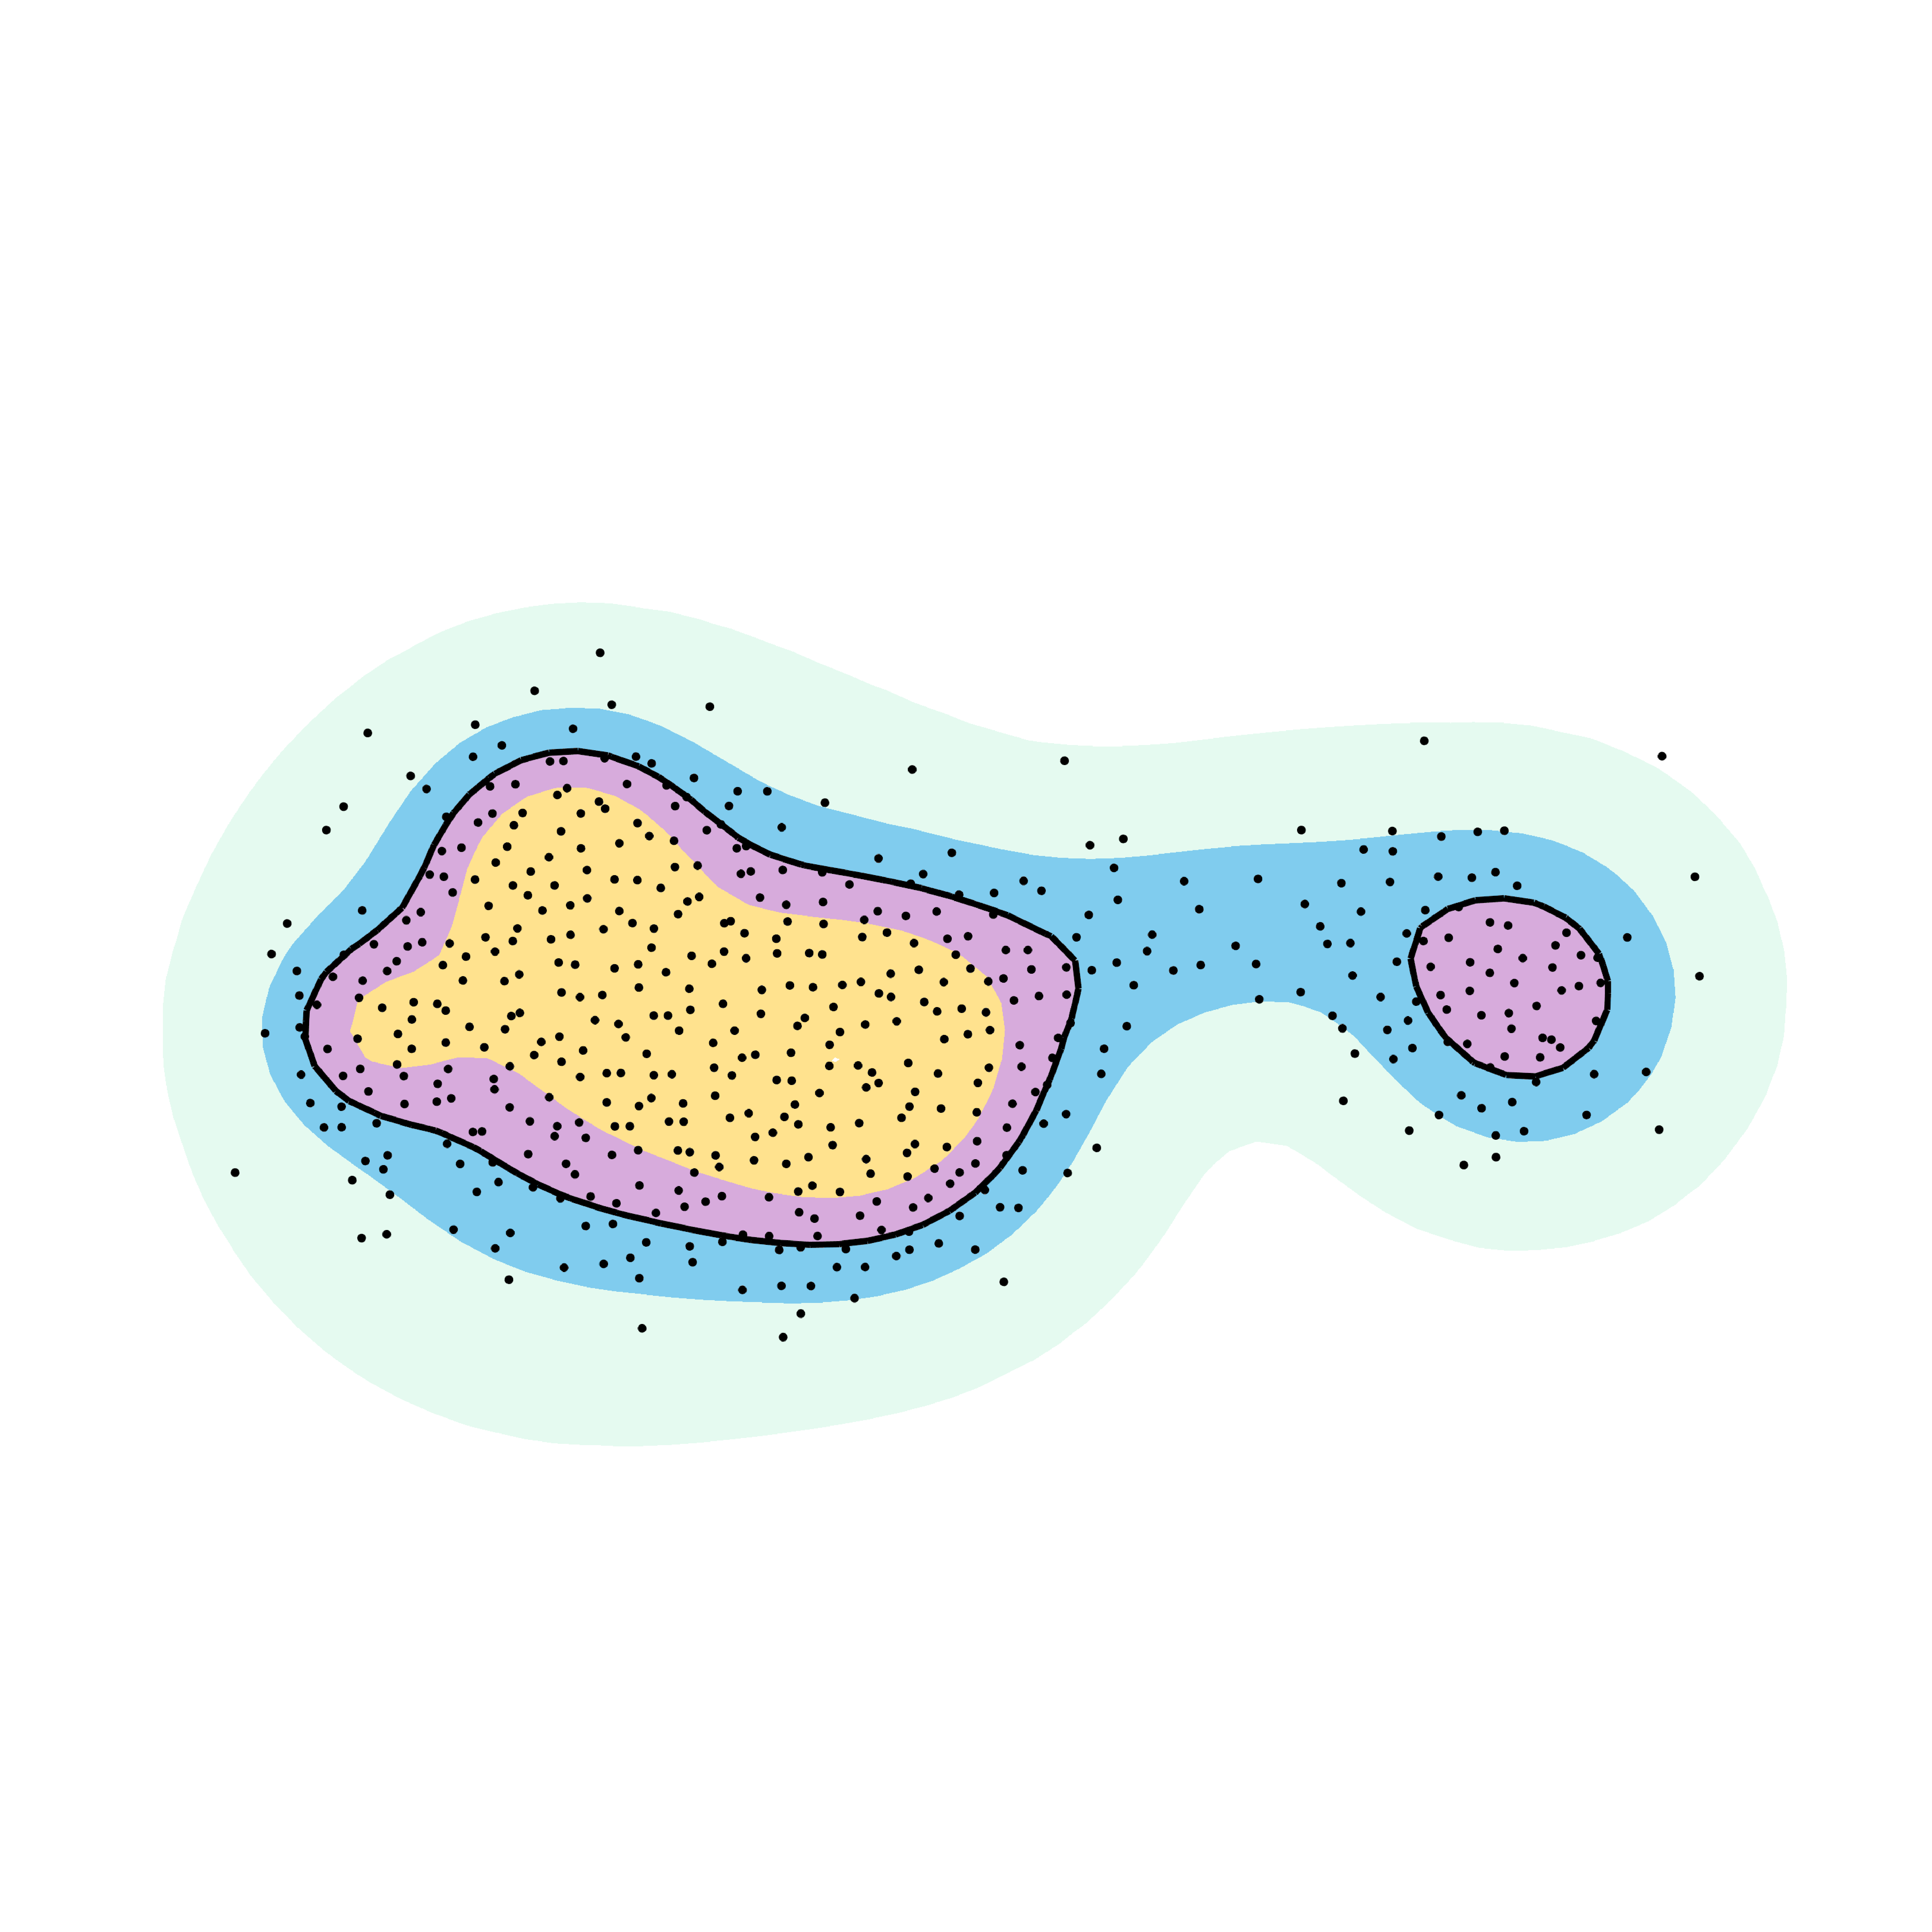
\includegraphics[trim=0 500 0 500, clip, width=0.45\textwidth]{figures/samples/samples_comp.pdf}
  % 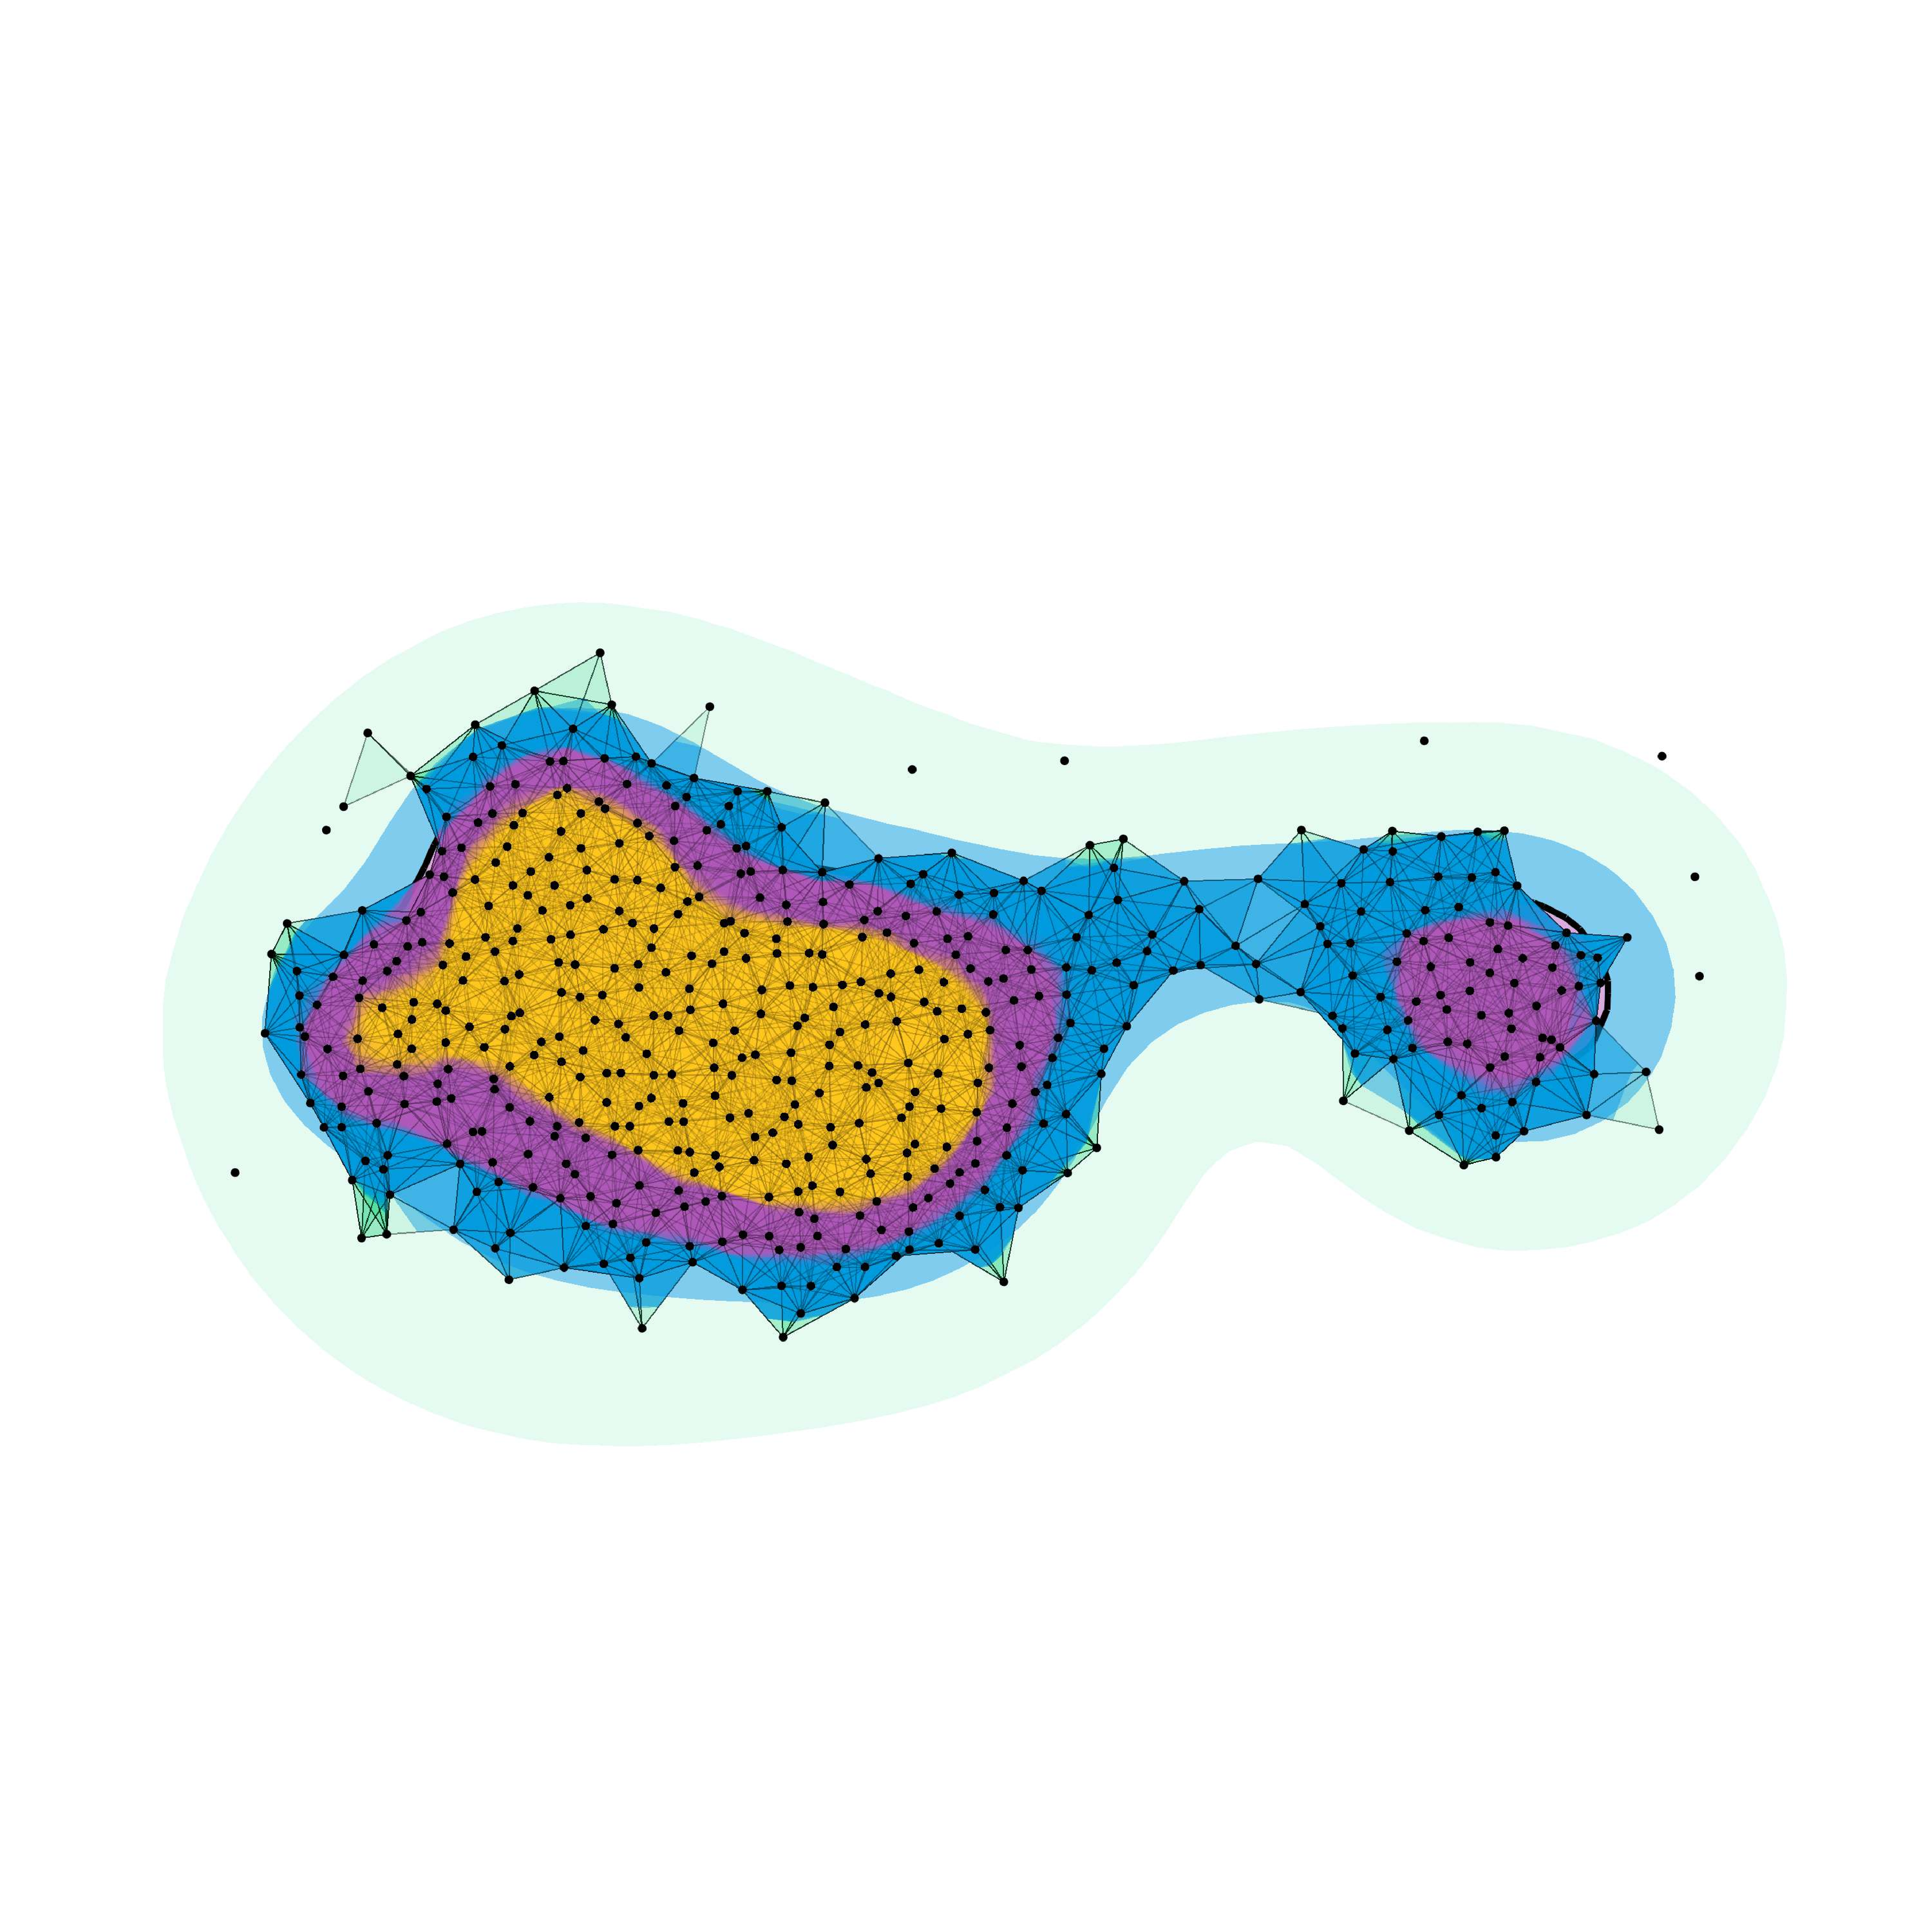
\includegraphics[trim=0 500 0 500, clip, width=0.45\textwidth]{figures/samples/scalar1_comp.pdf}
  % 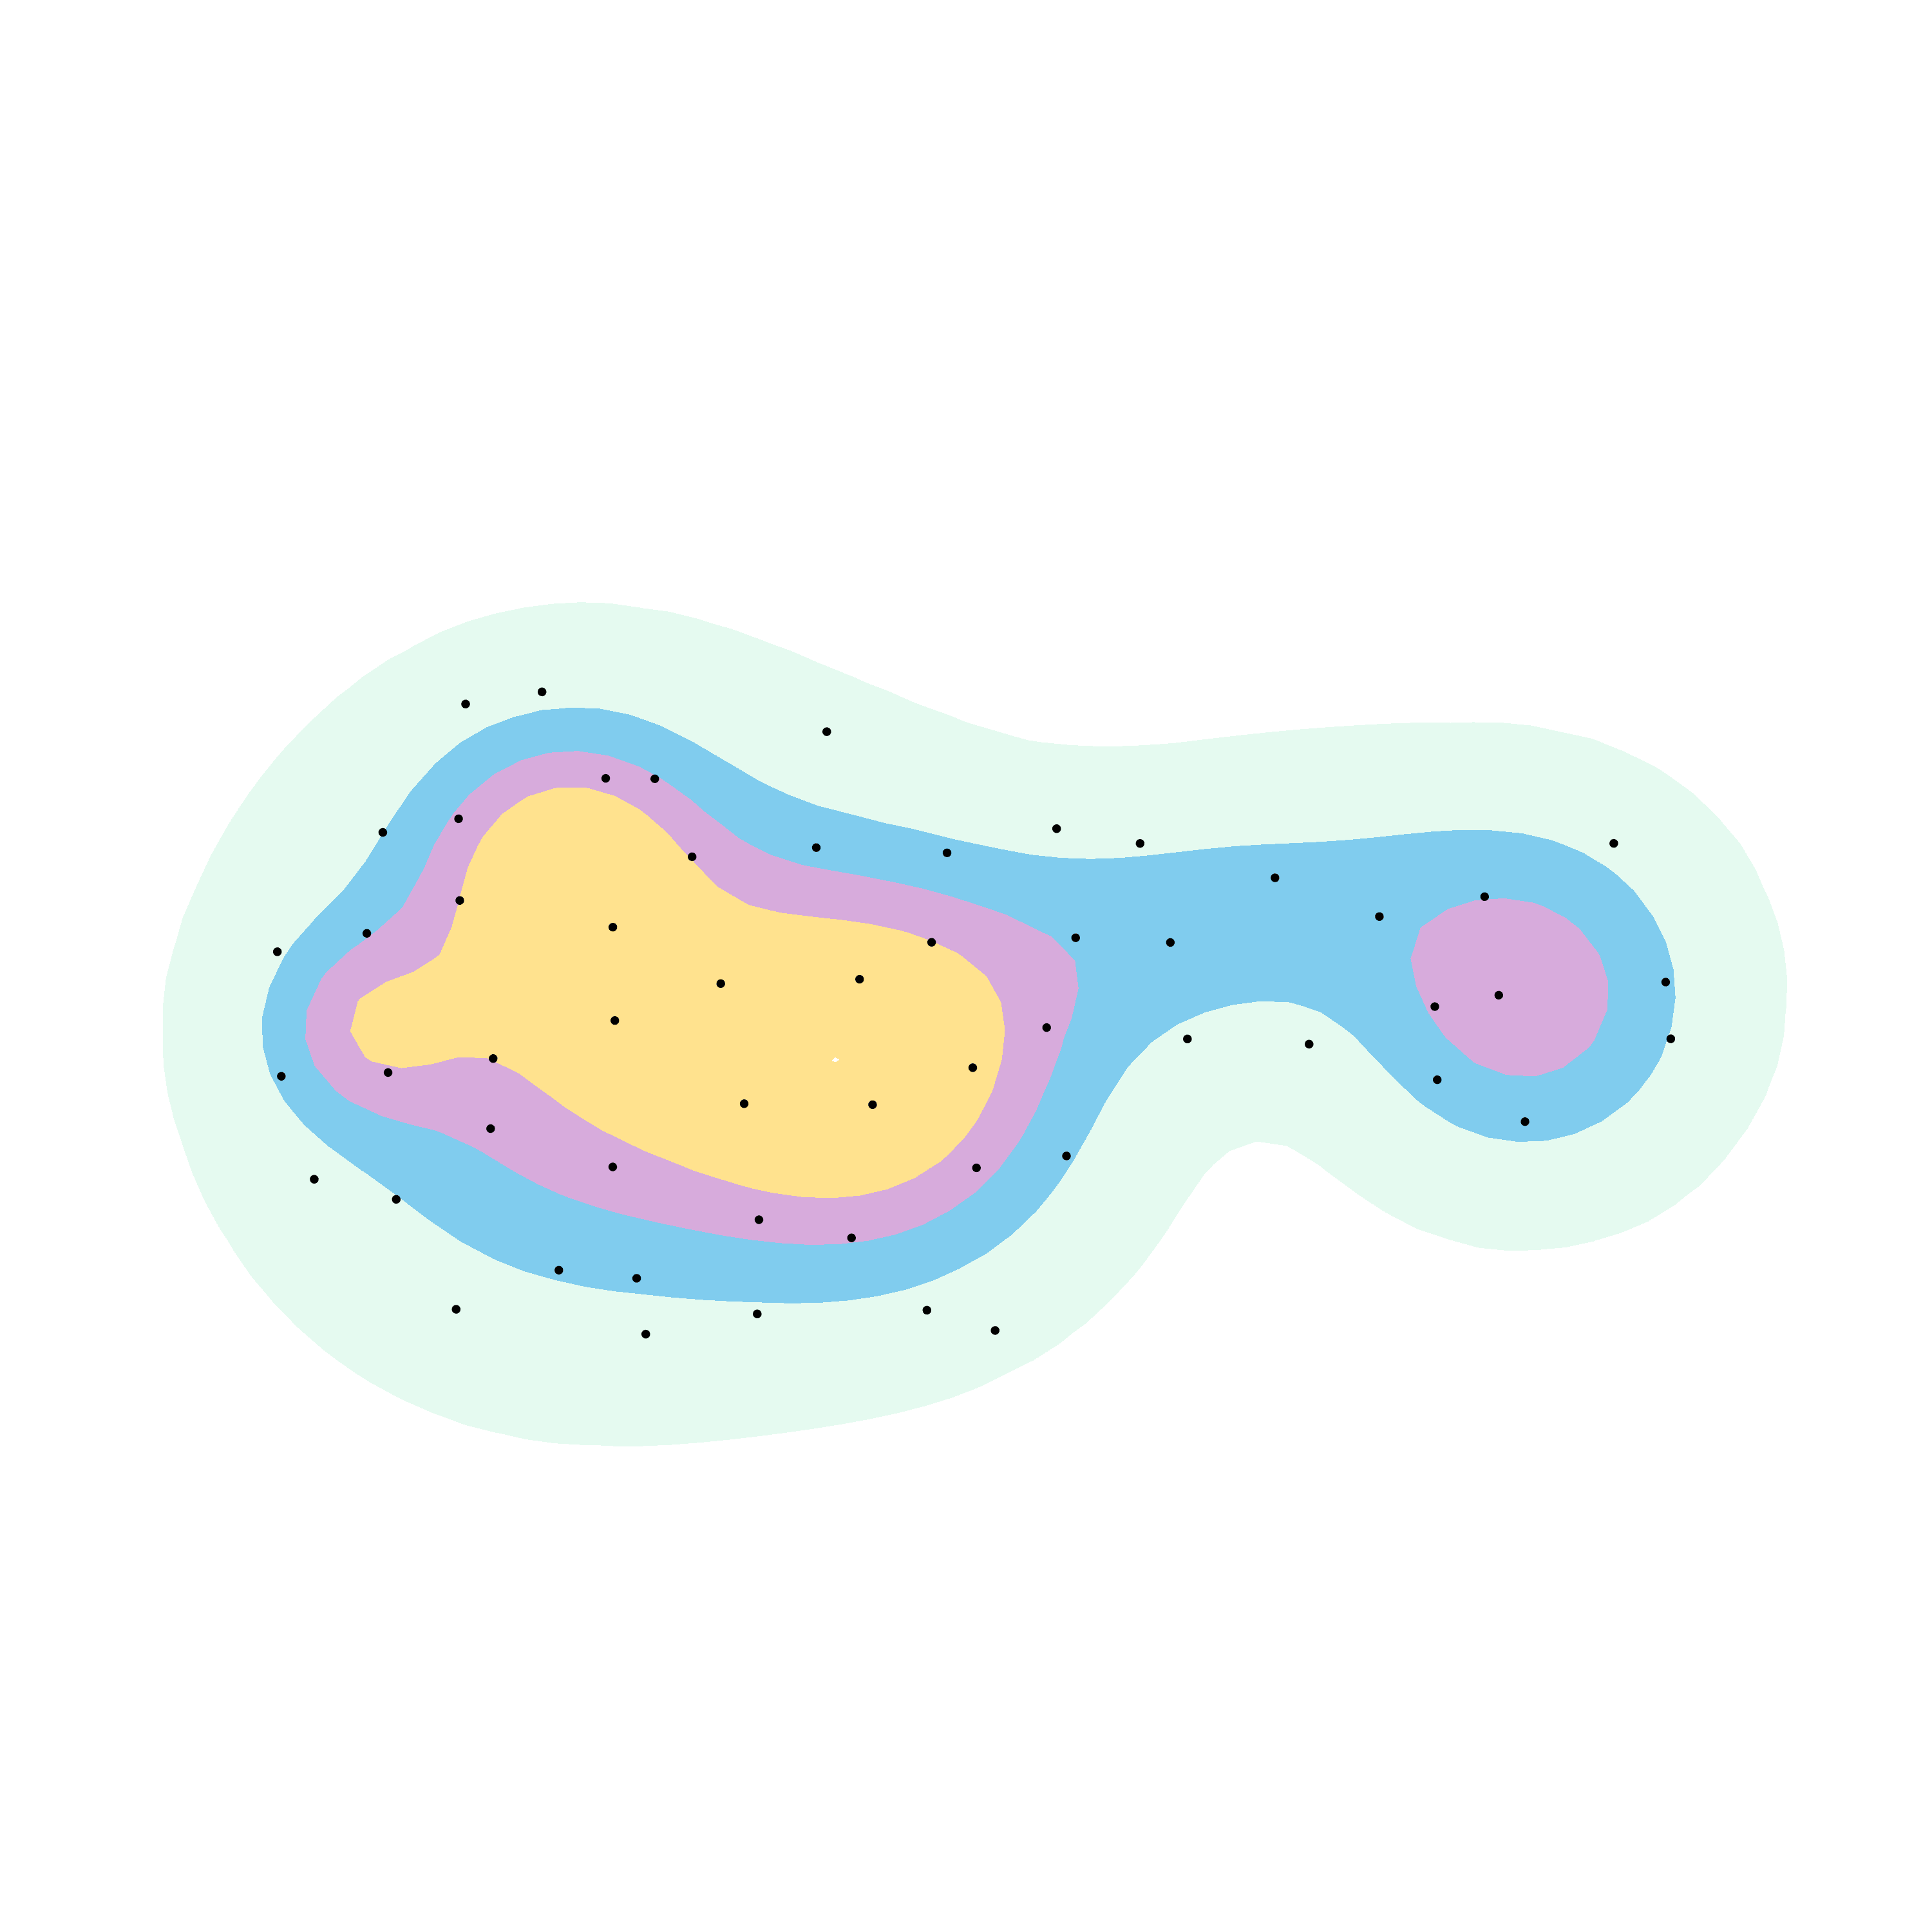
\includegraphics[trim=0 500 0 500, clip, width=0.45\textwidth]{figures/partial5/samples}
  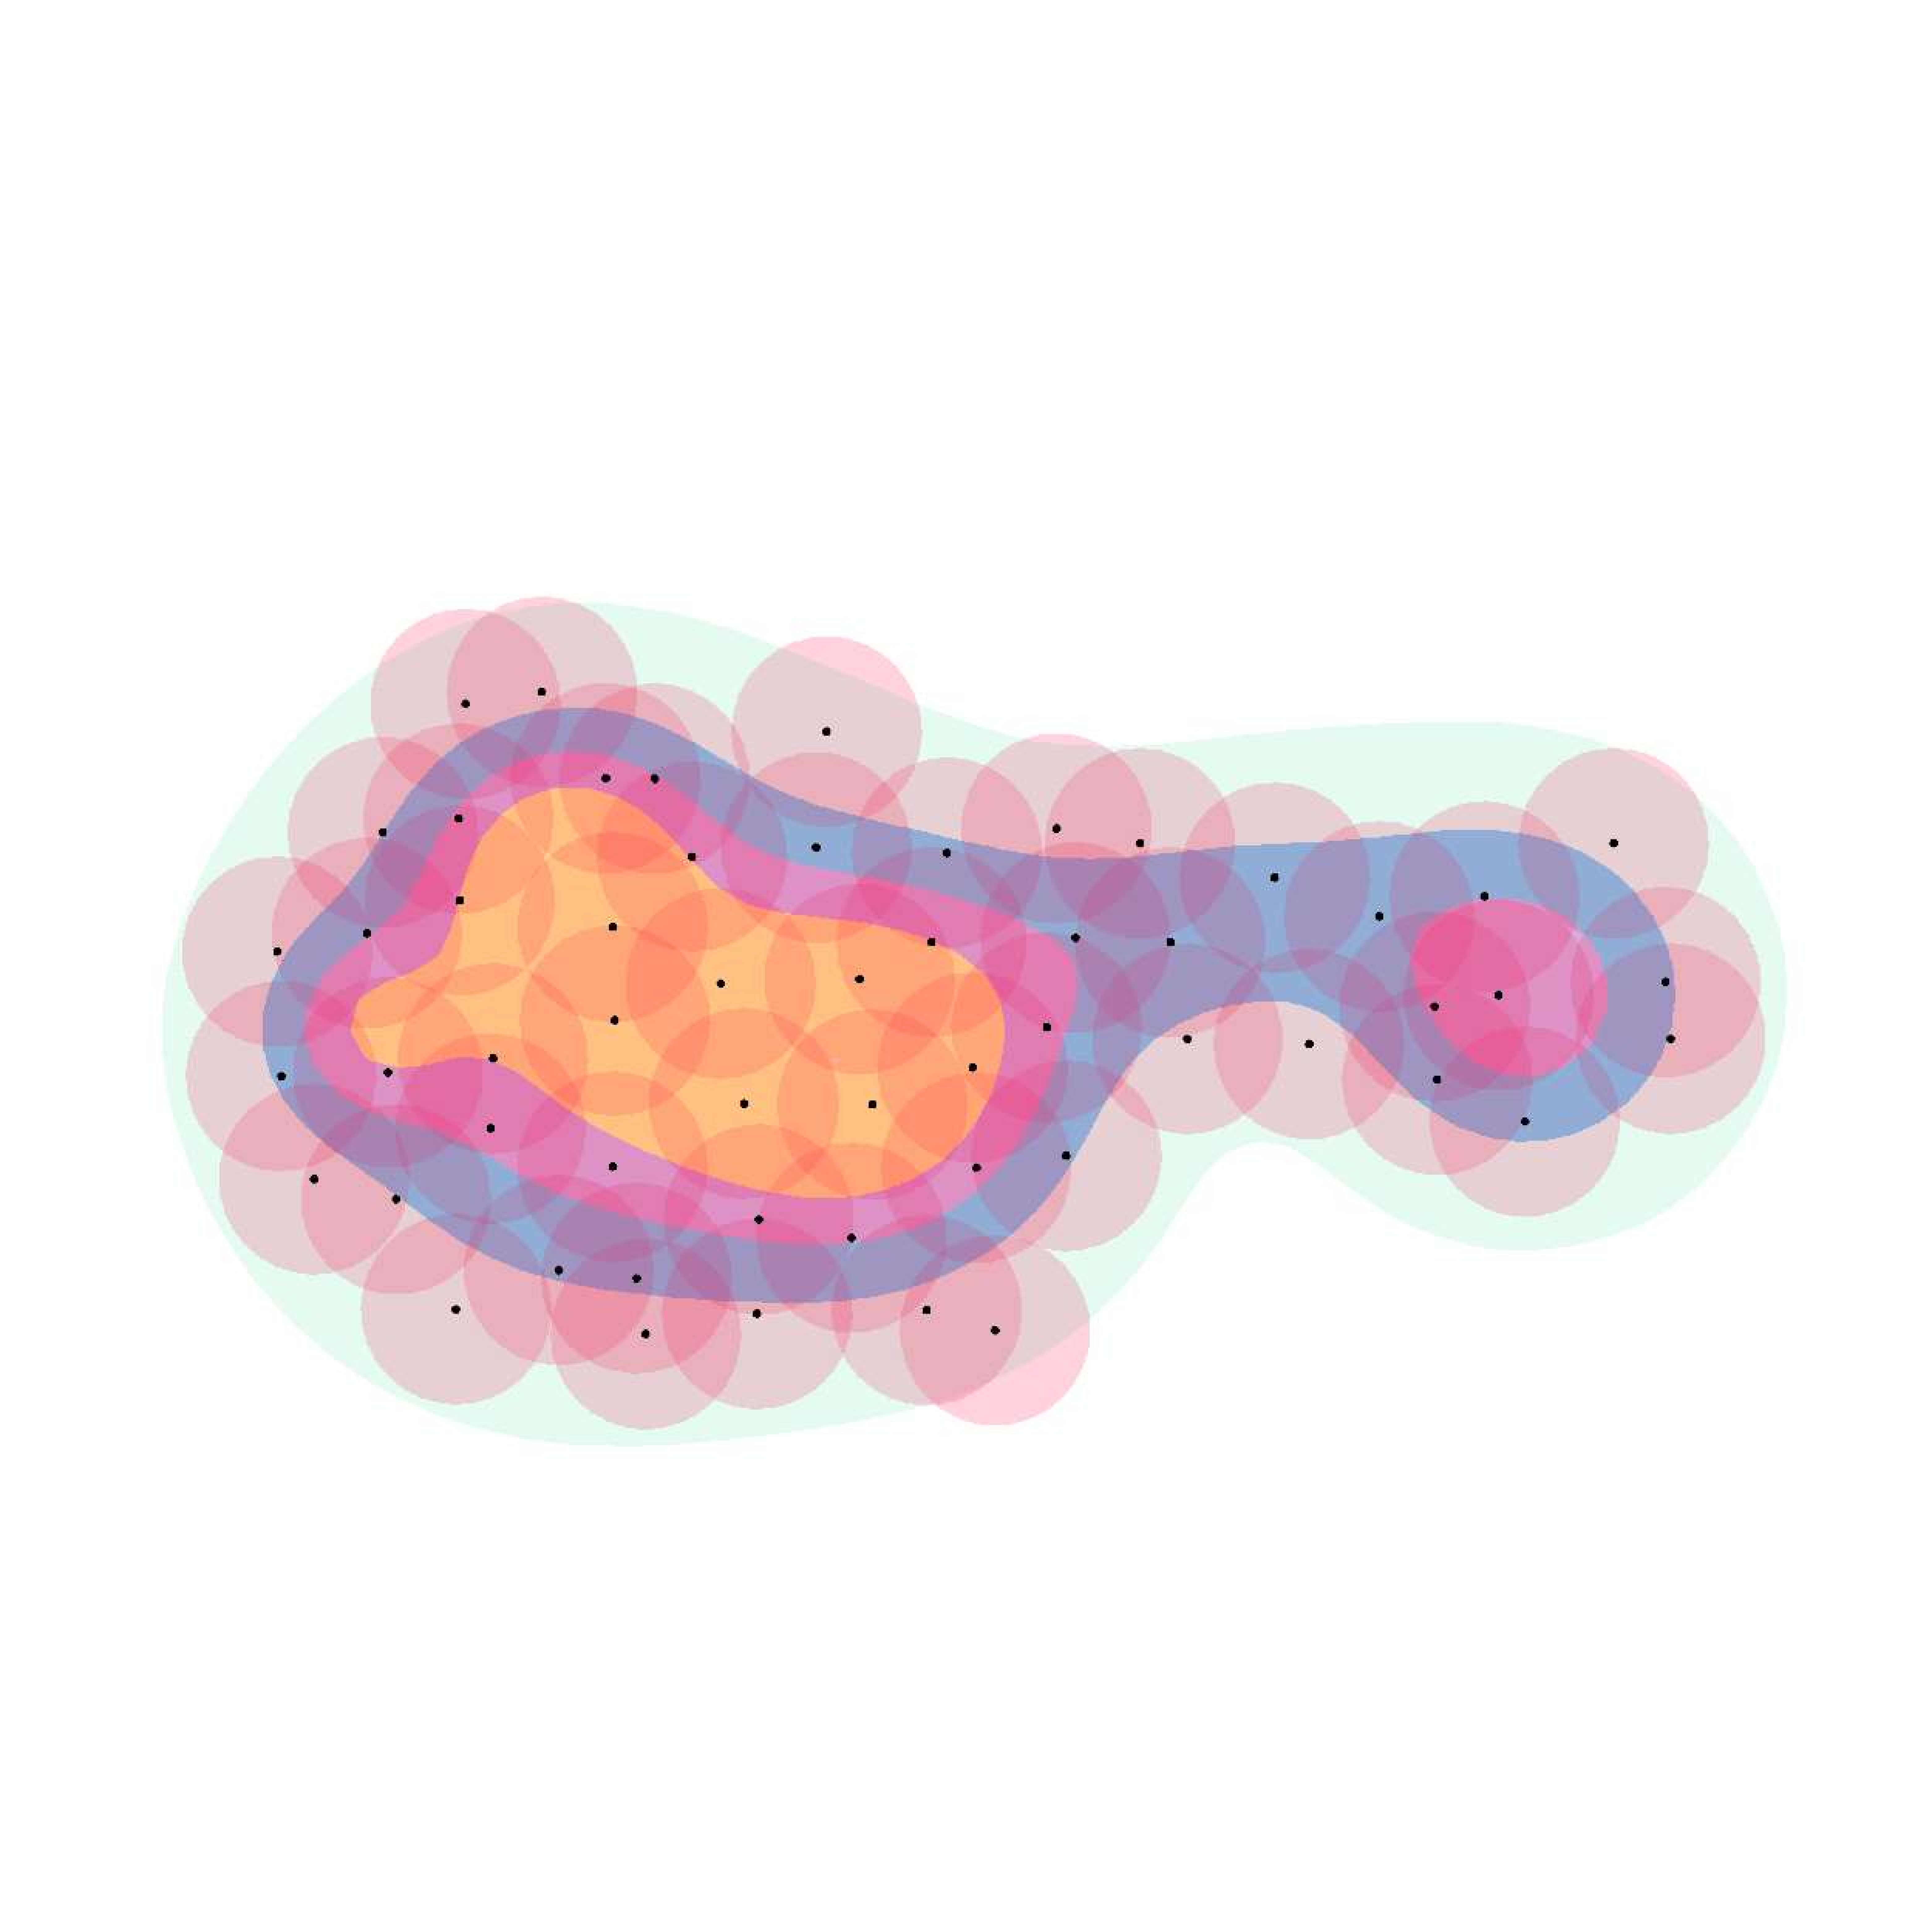
\includegraphics[trim=0 500 0 500, clip, width=0.45\textwidth]{figures/partial5/cover-comp.pdf}
  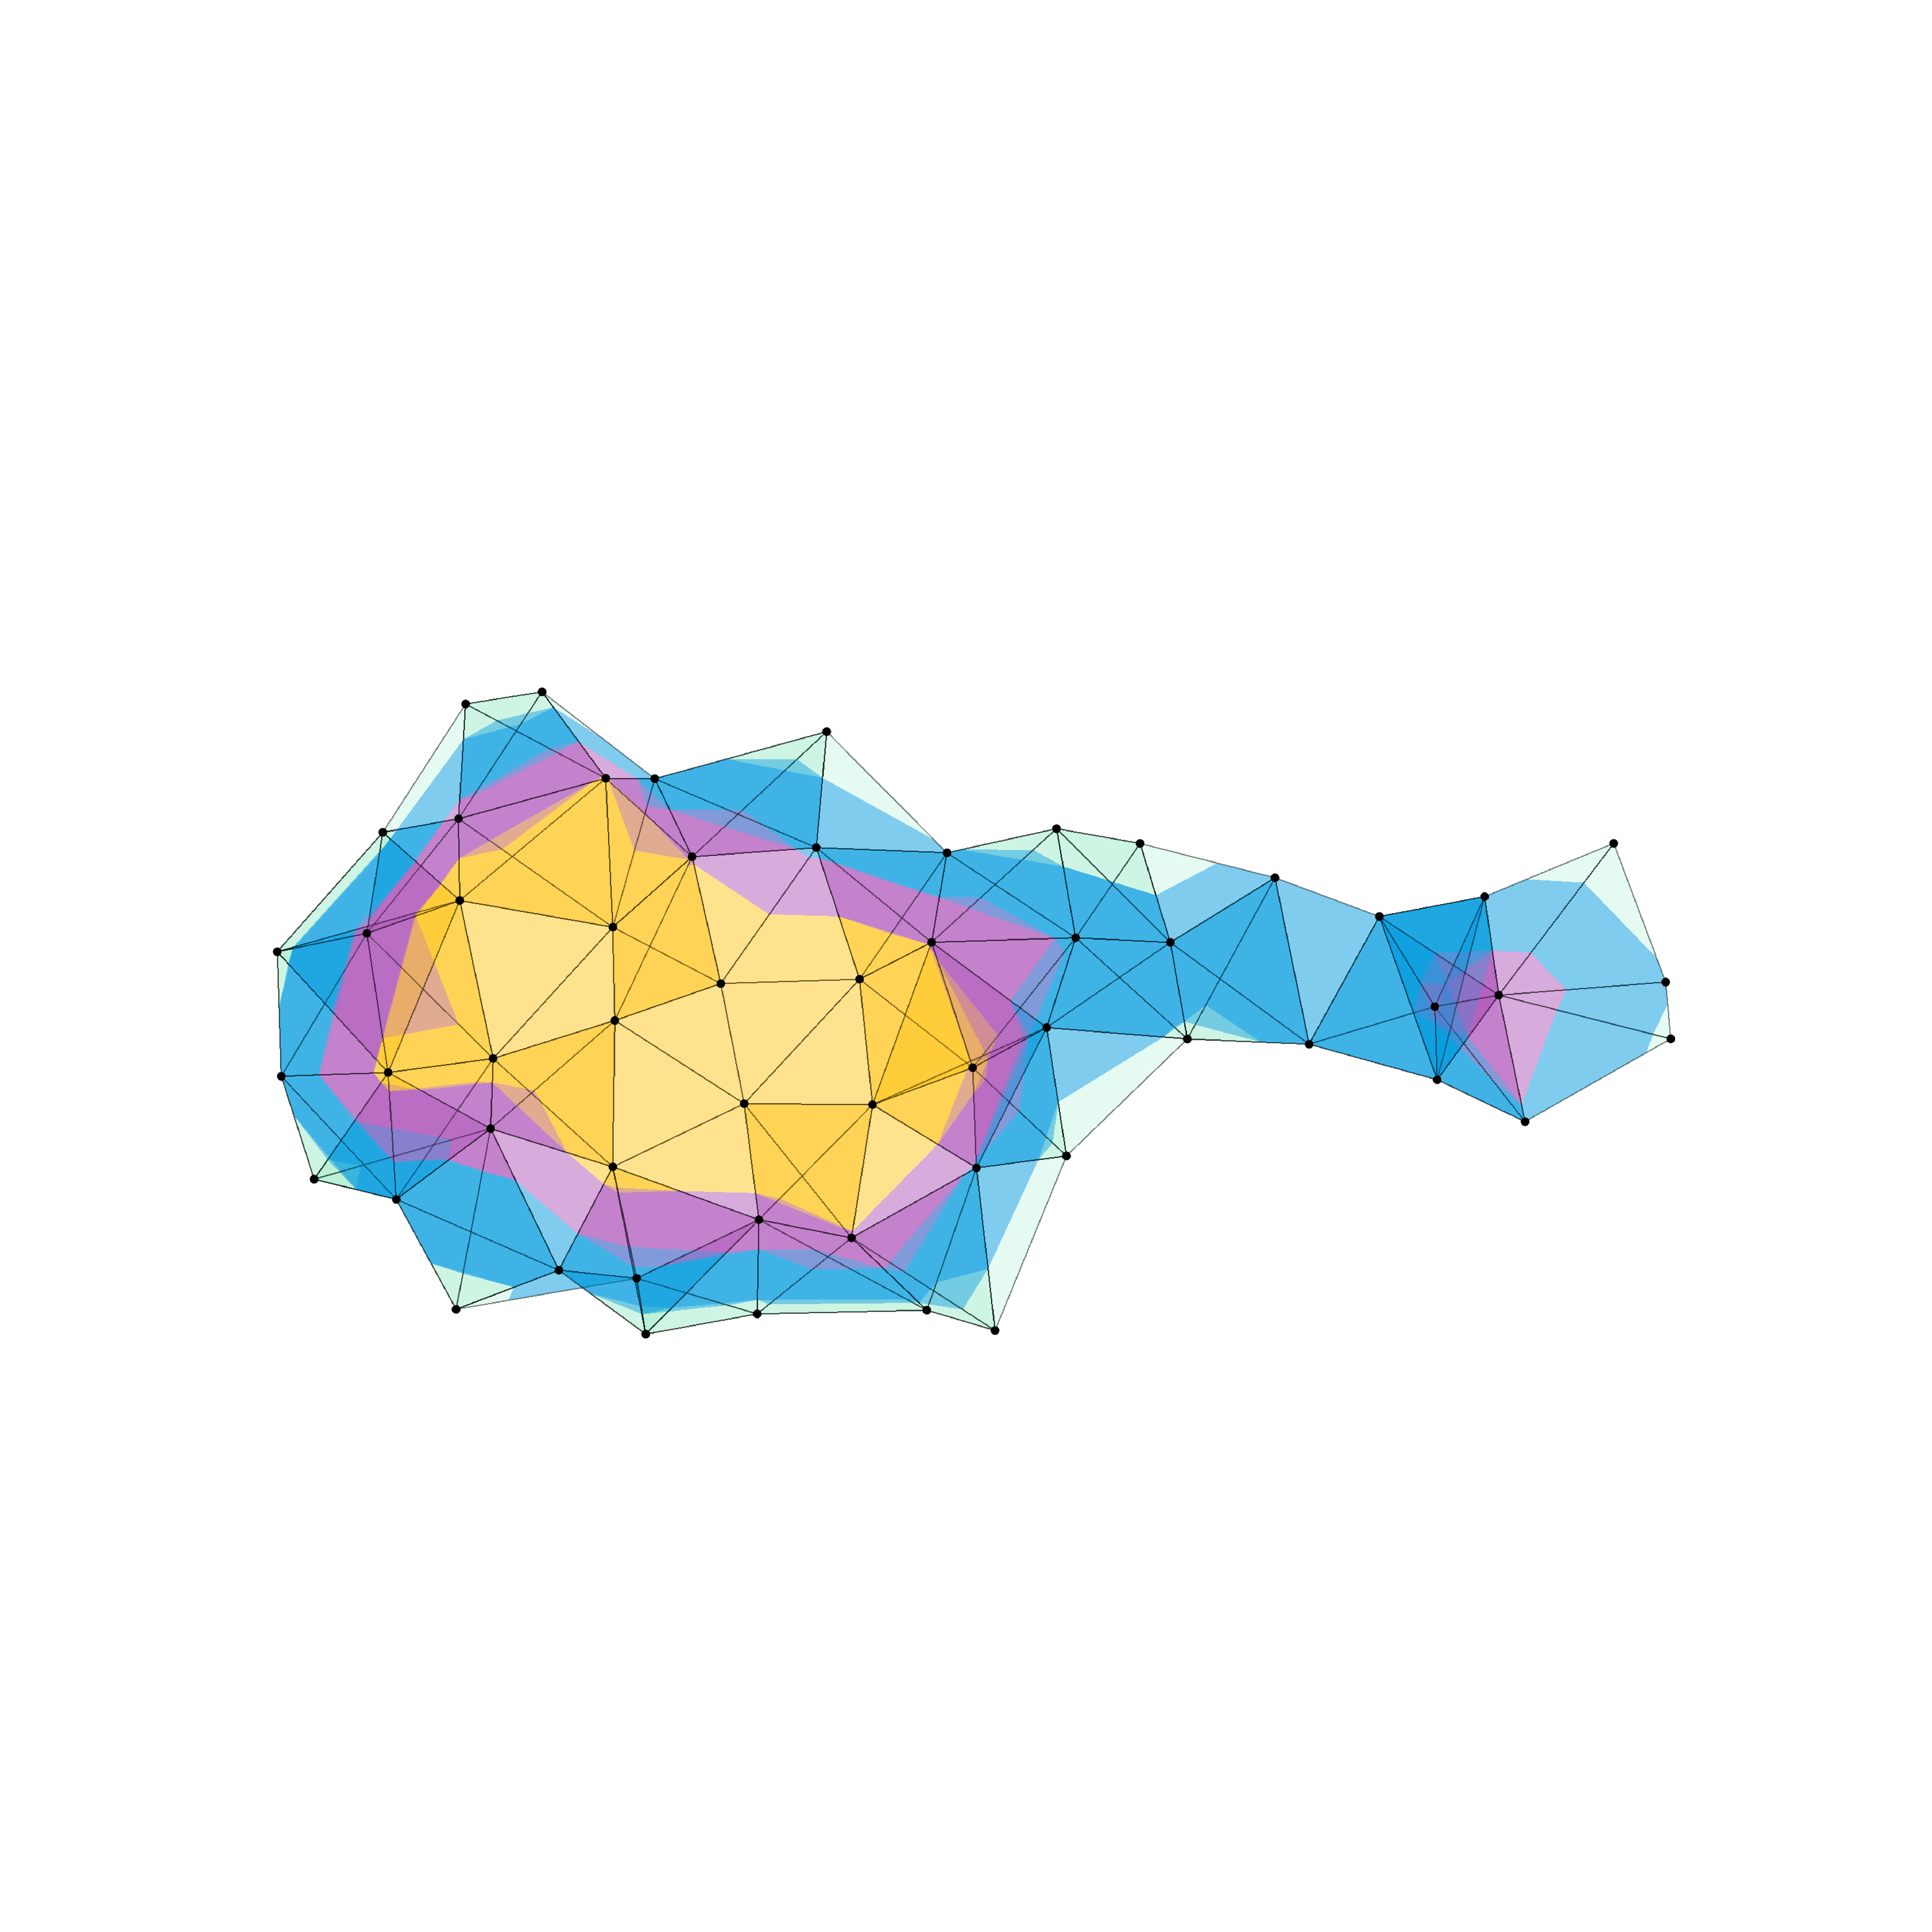
\includegraphics[trim=0 500 0 500, clip, width=0.45\textwidth]{figures/partial5/complex_nosurf.pdf}
  \caption{A partially sampled scalar field.}\label{fig:main}
\end{figure}

We will begin by reviewing relevant background information in geometry and topology.
We will then introduce the notion of a surrounding pair and prove an important property that generalizes part of the traditional proof of the TCC.
We will then apply this property to the geometric case before showing how it can be computed.

%
% Connected components, loops, and voids are examples of topological invariants that correspond to ``holes'' in dimensions 0, 1, and 2.
% These invariants can be computed using a tool from algebraic topology known as \emph{homology}.
% Homology not only quantifies these holes but also associates an algebraic structure to the space in each dimension.
% Given a scalar valued function on the spae persistent homology uses this structure to decompose its homology in a way that provides useful geometric and topological information about both the function and the space itself.
%
% Persistent homology is a central tool in the emerging field of Topological Data Analysis (TDA) which is concerned with the ``shape of data.''
% TDA has found a number of applications in\ldots
% The appeal of topological methods in data analysis is primarily due to their ability to identify meaningful global structure from local data in high dimensions.
% Often this analysis involves approximating the persistent homology of a scalar valued function on some unknown domain from a set of sample points.
% We refer to this approximation as Topological Scalar Field Analysis (SFA).
% A fundamental assumption required for strong guarantees is that the sample covers the domain of the function at a certain scale.
% % A fundamental assumption of this Topological Scalar Field Analysis (SFA) is that the sample sufficiently covers the domain of the function.
% The Topological Coverage Criterion (TCC) is a computable condition for coverage that uses the same homological and combinatorial tools required for SFA.
% We therefore present the TCC as a way to verify that a given sample is sufficient for SFA.
% Moreover, this reinterpretation allows us to extend SFA to the case of partial coverage.
%
% % Topology is the study of shape.
% % Topological data analysis (TDA) studies the shape of data.
% % This qualatative and quantitative information can provide insight on the structure of high dimensional data.
% % A key component of TDA is the analysis of scalar fields by persistent homology.
% % Homology is a tool from algebraic topology can identifies topological invariants, commonly referred to as ``holes,'' in arbitrary dimension.
% % Persistent homology tracks the evolution of these invariants over time.
% % {\color{red} The persistent homology of a scalar valued function provides a signature for the structure of the domain that maps to increasing sublevel sets. \textbf{why is this useful.}}
% % Given a collection of points that sample the function, one can approximate this signature with some guarantees.
% % Key to this is the requirement that the sample covers the domain of the function geometrically.
% % The topological coverage criterion uses these same homological and combinatorial tools to do just this---provide a computatible condition for coverage requiring only pairwise connectivity information.
% % Unlike previous work that requires the sample points can ``detect'' the presence of the true topological boundary we re-cast the TCC in a way that embraces the sample as that of a function.
% % That is, we will use the function values to identify a boundary as a sublevel set of the function, resolving one of the major barriers to wider use.
% % Moreover, this allows us to extend topological scalar field analysis to instances with partial coverage.
%
% % The topological coverage criterion (TCC) can be used to test whether an underlying space is sufficiently well covered by a given data set.
% % Given a sufficiently dense sample, topological scalar field analysis (SFA) can give a summary of the shape of a real-valued function on its domain.
% % The calculation and use of this summary is the subject of Topological Data Analysis (TDA) which is concerned with the ``shape'' of data.
% % The goal of this paper is to adapt the TCC so that one can test for coverage while computing a summary with SFA.
% % This provides a pipeline for verified scalar field analysis that simultaneously computes a topological signature of a function while testing that the underlying space is sufficiently well-sampled.
% %
% %
% % We will give a computable condition that ensures a set of sample points can be used to analyze the structure of a scalar field.
% % In other words, a way to verify that a given sample can provide a signature that captures both qualitative and quantitative shape information from a set of points endowed with a metric and a real-valued function.
% % % The only requirement is that these points are endowed with limited pairwise connectivity information.
% % In comparison to previous work our approach embraces the sample as that of a scalar-valued function, resolving one of the major barriers to wider use.
% %
% % Topological scalar field analysis is concerned with the properties of a space through the lens of a real-valued function.
% % We consider a collection of points along with only
%
% Initiated by De Silva and Ghrist~\cite{desilva06coordinate,desilva07coverage,desilva07homological}, the theory of homological sensor networks addresses the problem of testing coverage of a bounded domain by a collection of sensors without coordinates.
% The main result is the topological coverage criterion, which, in its most general form, states that under reasonable geometric assumptions, the $d$-dimensional relative homology of a pair of simplicial complexes built on the neighborhood graph will be nontrivial if and only if there is sufficient coverage (see Section~\ref{sec:tcc} for the precise statements).
% This relative persistent homology test is called the Topological Coverage Criterion (TCC).
% Prior work on SFA by Chazal et al.~\cite{chazal09analysis} showed that for sufficiently dense samples on sufficiently smooth spaces, the persistence diagram can be computed with some guarantees.
% In followup work, Buchet et al.~\cite{buchet15topological} extended this result to show how to work with noisy inputs.
%
% Superficially, the methods of SFA and TCC are very similar.
% Both construct similar complexes and compute the persistent homology of the homological image of a complex on one scale into that of a larger scale.
% They even overlap on some common techniques in their analysis such as the use of the Nerve theorem and the Rips-\v{C}ech interleaving.
% However, they differ in some fundamental ways that make them difficult to combine as a single technique.
% The main difference is that the TCC requires a clearly defined boundary.
% Not only must the underlying space be a bounded subset of $\R^d$, the data must also be labeled to indicate which input points are close to the boundary.
% This requirement is perhaps the main reason why the TCC can so rarely be applied in practice.
% % Cavanna et al.~\cite{cavanna2017when} generalized the TCC to allow for more general spaces and robust coverage guarantees.
% % That work gave a different approach to proving the correctness of the TCC which allows much more freedom in how the boundary is defined.
%
% In applications to data analysis it is more natural to assume that the data measures some unknown function.
% % By requiring that our function is related to the metric of the space
% We can then replace this requirement with assumptions about the function itself.
% Indeed, these assumptions could relate the behavior of the function to the topological boundary of the space.
% However, the generalized approach by Cavanna et al.~\cite{cavanna2017when} allows much more freedom in how the boundary is defined.
%
% We consider the case in which we have incomplete data from a particular sublevel set of our function.
% % We consider the case where we can only verify our sample in a part of the  % have incomplete data from a particular sublevel set of our function.
% Our goal is to isolate this data so we can analyze the function in only the verified region.
% %corresponding part persistent homology of the function in the verified region without allowing missing
% From this perspective, the TCC confirms that we not only have coverage, but that the sample we have is topologically representative of the region near, and above this sublevel set.
% We can then re-use the same machinery to analyze a \emph{part} of the function in a specific way.
